% !TeX spellcheck = sl_SI
% vim: set spell spelllang=sl:
% za preverjanje črkovanja, če se uporablja Texstudio ali vim
\documentclass[12pt,a4paper,twoside]{article}
\usepackage[utf8]{inputenc}  % pravilno razpoznavanje unicode znakov

% NASLEDNJE UKAZE USTREZNO POPRAVI
\newcommand{\program}{Matematika} % ime studijskega programa
\newcommand{\imeavtorja}{Tjaša Vrhovnik} % ime avtorja
\newcommand{\imementorja}{prof.~dr.~Franc Forstnerič} % akademski naziv in ime mentorja, uporabi poln naziv, prof.~dr.~, doc.~dr., ali izr.~prof.~dr.
\newcommand{\imesomentorja}{} % akademski naziv in ime somentorja, če ga imate
\newcommand{\naslovdela}{Minimalne ploskve}
\newcommand{\letnica}{2021} % letnica magistriranja
\newcommand{\opis}{}  % Opis dela v eni povedi. Ne sme vsebovati matematičnih simbolov v $ $.
\newcommand{\kljucnebesede}{} % ključne besede, ločene z \sep, da se PDF metapodatki prav procesirajo
\newcommand{\keywords}{} % ključne besede v angleščini
\newcommand{\organization}{Univerza v Ljubljani, Fakulteta za matematiko in fiziko} % fakulteta
\newcommand{\literatura}{literatura}  % pot do datoteke z literaturo (brez .bib končnice)
\newcommand{\sep}{, }  % separator med ključnimi besedami v besedilu
% KONEC PODATKOV

\usepackage{bibentry}         % za navajanje literature v programu dela s celim imenom
\nobibliography{\literatura}
\newcommand{\plancite}[1]{\item[\cite{#1}] \bibentry{#1}} % citiranje v programu dela

\usepackage{filecontents}  % za pisanje datoteke s PDF metapodatki
\usepackage{silence} \WarningFilter{latex}{Overwriting file}  % odstrani annoying warning o obstoju datoteke
% datoteka s PDF metapodatki, zgenerira se kot magisterij.xmpdata
\begin{filecontents*}{\jobname.xmpdata}
  \Title{\naslovdela}
  \Author{\imeavtorja}
  \Keywords{\kljucnebesede}
  \Subject{matematika}
  \Org{\organization}
\end{filecontents*}

\usepackage[a-1b]{pdfx}  % zgenerira PDF v tem PDF/A-1b formatu, kot zahteva knjižnica
\hypersetup{bookmarksopen, bookmarksdepth=3, colorlinks=true,
  linkcolor=black, anchorcolor=black, citecolor=black, filecolor=black,
  menucolor=black, runcolor=black, urlcolor=black, pdfencoding=auto,
  breaklinks=true, psdextra}

\usepackage[slovene]{babel}  % slovenščina
\usepackage[T1]{fontenc}     % naprednejše kodiranje fonta
\usepackage{amsmath,amssymb,amsfonts,amsthm} % matematični paketi
\usepackage{graphicx}     % za slike
\usepackage{emptypage}    % prazne strani so neoštevilčene, ampak so štete
\usepackage{units}        % fizikalne enote kot \unit[12]{kg} s polovico nedeljivega presledka, glej primer v kodi
\usepackage{makeidx}      % za stvarno kazalo, lahko zakomentiraš, če ne rabiš
\makeindex                % za stvarno kazalo, lahko zakomentiraš, če ne rabiš
% oblika strani
\usepackage[
  top=3cm,
  bottom=3cm,
  inner=3.5cm,      % margini za dvostransko tiskanje
  outer=2.5cm,
  footskip=40pt     % pozicija številke strani
]{geometry}

% VEČ ZANIMIVIH PAKETOV
% \usepackage{array}      % več možnosti za tabele
% \usepackage[list=true,listformat=simple]{subcaption}  % več kot ena slika na figure, omogoči slika 1a, slika 1b
% \usepackage[all]{xy}    % diagrami
% \usepackage{doi}        % za clickable DOI entrye v bibliografiji
% \usepackage{enumerate}     % več možnosti za sezname

% Za barvanje source kode
% \usepackage{minted}
% \renewcommand\listingscaption{Program}

% Za pisanje psevdokode
% \usepackage{algpseudocode}  % za psevdokodo
% \usepackage{algorithm}
% \floatname{algorithm}{Algoritem}
% \renewcommand{\listalgorithmname}{Kazalo algoritmov}

% DRUGI TVOJI PAKETI:
% tukaj

\setlength{\overfullrule}{50pt} % označi predlogo vrstico
\pagestyle{plain}               % samo številka strani na dnu, nobene glave / noge

% ukazi za matematična okolja
\theoremstyle{definition} % tekst napisan pokončno
\newtheorem{definicija}{Definicija}[section]
\newtheorem{primer}[definicija]{Primer}
\newtheorem{opomba}[definicija]{Opomba}
\newtheorem{aksiom}{Aksiom}

\newenvironment{dokaz}[1][Dokaz]{\begin{proof}[#1]}{\end{proof}}

\theoremstyle{plain} % tekst napisan poševno
\newtheorem{lema}[definicija]{Lema}
\newtheorem{izrek}[definicija]{Izrek}
\newtheorem{trditev}[definicija]{Trditev}
\newtheorem{posledica}[definicija]{Posledica}

\numberwithin{equation}{section}  % števec za enačbe zgleda kot (2.7) in se resetira v vsakem poglavju

% Matematični ukazi
\newcommand{\R}{\mathbb R}
\newcommand{\N}{\mathbb N}
\newcommand{\Z}{\mathbb Z}
%\renewcommand{\C}{\mathbb C}
\newcommand{\C}{\mathbb C}
\newcommand{\Q}{\mathbb Q}

% \DeclareMathOperator{\tr}{tr}  % morda potrebuješ operator za sled ali kaj drugega?

% bold matematika znotraj \textbf{ }, tudi v naslovih, kot \omega spodaj
\makeatletter \g@addto@macro\bfseries{\boldmath} \makeatother

% Poimenuj kazalo slik kot ``Kazalo slik'' in ne ``Slike''
\addto\captionsslovene{
  \renewcommand{\listfigurename}{Kazalo slik}%
}

% če želiš, da se poglavja začnejo na lihih straneh zgoraj
% \let\oldsection\section
% \def\section{\cleardoublepage\oldsection}

%%%%%%%%%%%%%%%%%%%%%%%%%%%%%%%%%%%%%%%%%%
%%%%%%           DOCUMENT           %%%%%%
%%%%%%%%%%%%%%%%%%%%%%%%%%%%%%%%%%%%%%%%%%

\begin{document}

\pagenumbering{roman} % začnemo z rimskimi številkami
\thispagestyle{empty} % ampak na prvi strani ni številke

\noindent{\large
UNIVERZA V LJUBLJANI\\[1mm]
FAKULTETA ZA MATEMATIKO IN FIZIKO\\[5mm]
\program\ -- 2.~stopnja}
% ustrezno dopolni za IŠRM
\vfill

\begin{center}
  \large
  \imeavtorja\\[3mm]
  \Large
  \textbf{\MakeUppercase{\naslovdela}}\\[10mm]
  \large
  Magistrsko delo \\[1cm]
  Mentor: \imementorja \\[2mm] % ustrezno popravi spol
%   Somentor: \imesomentorja   % dodaj, če potrebno
\end{center}
\vfill

\noindent{\large Ljubljana, \letnica}

\cleardoublepage

%% sem pride IZJAVA O AVTORSTVU  -- SE NATISNE V VIS

% zahvala
\pdfbookmark[1]{Zahvala}{zahvala} %
\section*{Zahvala}
% end zahvala -- izbriši vse med zahvala in end zahvala, če je ne rabiš

\cleardoublepage

\pdfbookmark[1]{\contentsname}{kazalo-vsebine}
\tableofcontents

% list of figures
% \cleardoublepage
% \pdfbookmark[1]{\listfigurename}{kazalo-slik}
% \listoffigures
% end list of figures

\cleardoublepage

\section*{Program dela}
\addcontentsline{toc}{section}{Program dela} % dodajmo v kazalo

\section*{Osnovna literatura}
Literatura mora biti tukaj posebej samostojno navedena (po pomembnosti) in ne
le citirana. V tem razdelku literature ne oštevilčimo po svoje, ampak uporabljamo
okolje itemize in ukaz plancite, saj je celotna literatura oštevilčena na koncu.
\begin{itemize}
  \plancite{lebedev2009introduction}
  \plancite{gurtin1982introduction}
  \plancite{zienkiewicz2000finite}
  \plancite{STtemplate}
\end{itemize}

\vspace{2cm}
\hspace*{\fill} Podpis mentorja: \phantom{prostor za podpis}

% \vspace{2cm}
% \hspace*{\fill} Podpis somentorja: \phantom{prostor za podpis}

\cleardoublepage
\pdfbookmark[1]{Povzetek}{abstract}

\begin{center}
\textbf{\naslovdela} \\[3mm]
\textsc{Povzetek} \\[2mm]
\end{center}
Tukaj napišemo povzetek vsebine. Sem sodi razlaga vsebine in ne opis tega, kako je delo
organizirano.

\vfill
\begin{center}
\textbf{English translation of the title} \\[3mm] % prevod slovenskega naslova dela
\textsc{Abstract}\\[2mm]
\end{center}

An abstract of the work is written here. This includes a short description of
the content and not the structure of your work.

\vfill\noindent
\textbf{Math.~Subj.~Class.~(2010):} oznake kot 74B05, 65N99, na voljo so na naslovu
\url{http://www.ams.org/msc/msc2010.html} \\[1mm]
\textbf{Ključne besede:} \kljucnebesede \\[1mm]
\textbf{Keywords:} \keywords

\cleardoublepage

\setcounter{page}{1}    % od sedaj naprej začni zopet z 1
\pagenumbering{arabic}  % in z arabskimi številkami

%%%%%%%%%%%%%%%%%%%%%%%%%%%%%%%%%%%%%%%%%%%%%%%%%%%%%%%%%%%%%%%%%%%%%%%%%%%%%
%%%%%%%%%%%%%%%%%%%%%%%%%%%%%%%%%%%%%%%%%%%%%%%%%%%%%%%%%%%%%%%%%%%%%%%%%%%%%
% Uvod
\section{Uvod}

%%%%%%%%%%%%%%%%%%%%%%%%%%%%%%%%%%%%%%%%%%%%%%%%%%%%%%%%%%%%%%%%%%%%%%%%%%%%%
%%%%%%%%%%%%%%%%%%%%%%%%%%%%%%%%%%%%%%%%%%%%%%%%%%%%%%%%%%%%%%%%%%%%%%%%%%%%%
% Osnovni pojmi
\section{Osnovni pojmi}

%%%%%%%%%%%%%%%%%%%%%%%%%%%%%%%%%%%%%%%%%%%%%%%%%%%%%%%%%%%%%%%%%%%%%%%%%%%%%
% Mnogoterosti
\subsection{Mnogoterosti}

\begin{definicija}
Naj bo $n \in \N$. Topološki prostor $M$ z lastnostmi:
\begin{enumerate}
\item $M$ je Hausdorffov,
\item $M$ je 2-števen,
\item $M$ je lokalno Evklidski prostor dimenzije $n$ (za vsak $p \in M$ obstajata odprta okolica $U \subset M$ in homeomorfizem $\phi \colon U \to V \subset \R^{n}$, kjer je $V$ odprta množica),
\end{enumerate}
imenujemo \emph{topološka mnogoterost} dimenzije $n$.
\end{definicija}

Na topološki mnogoterosti $M$ dimenzije $n$ definiramo \emph{atlas} $\mathcal{U} = \{ (U_{i}, \phi_{i}) ; \ i \in I \}$ kot družino parov $(U_{i}, \phi_{i})$, kjer je $\{ U_{i} \}_{i \in I}$ odprto pokritje mnogoterosti $M$, preslikave $\phi_{i} \colon U_{i} \to \phi_{i}(U_{i}) \subset \R^{n}$ pa so homeomorfizmi za vse $i$. Par $(U_{i}, \phi_{i})$ imenujemo \emph{lokalna karta}.
Vzemimo lokalni karti $(U_{i}, \phi_{i})$ in $(U_{j}, \phi_{j})$, $i \neq j$, za kateri velja $U_{ij}=U_{i} \cap U_{j} \neq \emptyset$. Difeomorfizmu $\phi_{ij} = \phi_{j} \circ \phi_{i}^{-1} \colon \phi_{i}(U_{ij}) \to \phi_{j}(U_{ij})$ med odprtima podmnožicama $\R^{n}$ pravimo \emph{prehodna preslikava} med lokalnima kartama. Atlas je razreda $\mathcal{C}^{r}$ za $r \geq 1$, kadar so prehodne preslikave med vsemi lokalnimi kartami difeomorfizmi razreda $\mathcal{C}^{r}$. V tem primeru rečemo, da je $M$ \emph{mnogoterost razreda} $\mathcal{C}^{r}$.
V posebnem gladek atlas določa gladko mnogoterost.

\begin{definicija}
Naj bo $X$ mnogoterost razreda $\mathcal{C}^{r}$ razsežnosti $\dim X = n$ in $M \subset X$ njena podmnožica. Če za vsako točko $p \in M$ obstaja lokalna karta $(U, \phi)$ glede na atlas $\mathcal{U}$ mnogoterosti $X$, tako da je preslikava $\phi \colon U \to V \subset \mathbb{R}^{n}$ homeomorfizem in velja $\phi (M \cap U) = V \cap (\mathbb{R}^{m} \times \{0\}^{n-m})$, potem $M$ imenujemo \emph{podmnogoterost} razreda $\mathcal{C}^{r}$ razsežnosti $\dim M = m$.
\end{definicija}

\begin{definicija}[Orientacija mnogoterosti]
Naj bo $M$ gladka mnogoterost in $\mathcal{U}$ pripadajoč gladek atlas. Lokalni karti $(U, \phi)$ in $(V, \psi)$ določata isto orientacijo na $M$, če za poljubno točko $p \in U \cap V \neq \emptyset$ velja $\det (d(\psi \circ \phi ^{-1})_{\phi (p)}) > 0.$ Kadar poljubni lokalni karti glede na izbrani atlas $\mathcal{U}$ določata isto orientacijo, pravimo, da je atlas $\mathcal{U}$ \emph{orientiran}. Nadalje je mnogoterost \emph{orientabilna}, če premore orientiran atlas. \emph{Orientacija} mnogoterosti $M$ je izbor maksimalnega orientiranega atlasa na $M$.
\end{definicija}

Definirati želimo še tangentni prostor mnogoterosti. Naj bo $M$ gladka mnogoterost in izberimo atlas $\mathcal{U} = \{ (U_{i}, \phi_{i}) ; \ i \in I \}$ na njej. Naj bo točka $p \in U_{i} \subset M$ za nek indeks $i$.  Gladki krivulji\footnote{Krivulja $\gamma_{j}$ je gladka, če je preslikava $ \phi_{i} \circ \gamma_{j} \colon (-\varepsilon, \varepsilon) \to \mathbb{R}^{n}$, $j=1,2,$ gladka v običajnem smislu.} 
$\gamma_{1}, \gamma_{2} \colon (-\varepsilon, \varepsilon) \to M$ sta \emph{ekvivalentni}, če izpolnjujeta pogoja
$\gamma_{1}(0) = \gamma_{2}(0) = p$ in $ \frac{d}{dt}|_{t=0} \phi_{i}(\gamma_{1}(t)) =  \frac{d}{dt}|_{t=0} \phi_{i}(\gamma_{2}(t))$ za vse $t \in (-\varepsilon, \varepsilon)$. Ekvivalenco krivulj označimo z $\gamma_{1} \sim \gamma_{2}$\footnote{Relacija $\sim$ je ekvivalenčna relacija.}.

\begin{definicija}
Naj bo $M$ mnogoterost in $p \in M$ točka na njej. \emph{Tangentni vektor} $v_{p}$ na $M$ v točki $p$ ustreza ekvivalenčnemu razredu $[\gamma]$ krivulje $\gamma \colon (-\varepsilon, \varepsilon) \to M$, za katero velja $\gamma (0) = p$.

Unija vseh tangentnih vektorjev na $M$ v točki $p$ določa \emph{tangentni prostor} $T_{p}M$ mnogoterosti $M$ v točki $p$.
\end{definicija}

Naj bosta $M$ in $N$ mnogoterosti dimenzij $\dim M = m$, $\dim N = n$ ($m, n \in \N$). Naj bo $r \geq 0$. Pravimo, da je zvezna preslikava $f \colon M \to N$ \emph{razreda $\mathcal{C}^{r}$ v točki} $p \in M$, če obstajata taki $\mathcal{C}^{r}$ karti $(U, \phi)$ na $M$ v okolici točke $p \in M$ in $(V, \psi)$ na $N$ v okolici točke $f(p) \in N$, da je preslikava $F = \psi \circ f \circ \phi^{-1}$ razreda $\mathcal{C}^{r}$ v okolici točke $\phi(p)$.
Če to velja za poljubno točko $p \in M$, je $f$ \emph{razreda $\mathcal{C}^{r}$}; pišemo $f \in  \mathcal{C}^{r}(M,N)$.

Vzemimo gladki (oz.~razreda $\mathcal{C}^{r}$, $r \geq 1$) mnogoterosti $M$ in $N$ ter točko $p \in M$. \emph{Diferencial} gladke (oz.~razreda $\mathcal{C}^{r}$) preslikave $f \colon M \to N$ je linearna preslikava $df \colon T_{p}M \to T_{f(p)}N$, definirana s predpisom
\begin{equation}
(df_{p})[\gamma] = [f \circ \gamma].
\end{equation}

\begin{definicija}
Naj bo $f \colon M \to N$ gladka preslikava med gladkima mnogoterostima. Preslikava $f$ se imenuje 
\begin{enumerate}
\item \emph{imerzija} v točki $p \in M$, če je njen diferencial $df_{p} \colon T_{p}M \to T_{f(p)}N$ injektiven;
\item \emph{submerzija} v točki $p \in M$, če je njen diferencial $df_{p}$ surjektiven;
\item \emph{lokalni difeomorfizem} v točki $p \in M$, če obtstajata taki okolici $U \subset M$ za $p$ in $V \subset N$ za $f(p)$, da je zožitev $f|_{U} \colon U \to V$ difeomorfizem;
\item \emph{vložitev}, če je $f$ injektivna preslikava in slika $f(M) \subset N$ podmnogoterost.
\end{enumerate}
\end{definicija}

\begin{opomba}
Z uporabo izreka o implicitni preslikavi dokažemo naslednje: Če je $f \colon M \to N$ submerzija v okolici točke $p \in U$ ($U \subset M$ odprta), potem je praslika $f^{-1}(f(p))$ podmnogoterost v $M$ razsežnosti $\dim M - \dim N$.
\end{opomba}

% Riemannova metrika & mnogoterost
\begin{definicija}
Naj bo $M$ gladka mnogoterost. Za vsako točko $p \in M$ definiramo simetrično pozitivno-definitno bilinearno preslikavo $g_{p} \colon T_{p}M \times T_{p}M \to \R$, ki je gladko odvisna od $p$. Družino preslikav $g_{p}$ imenujemo \emph{Riemannova metrika} $g$ na mnogoterosti $M$.
Gladki mnogoterosti, opremljeni z Riemannovo metriko, pravimo \emph{Riemannova mnogoterost}, in jo označimo z $(M,g)$.
\end{definicija}

Izkaže se, da vsaka mnogoterost razreda $\mathcal{C}^{r+1}$ premore Riemannovo metriko razreda $\mathcal{C}^{r}$.

Naj bo $M$ domena v $\R^{n}$ s koordinatami $x = (x_{1}, \dots, x_{n})$. Riemannova metrika na $M$ je tedaj oblike
\begin{align}
g_{p} = \sum_{i,j=1}^{n} g_{i,j}(p) dx_{i} dx_{j}, \quad p \in M,
\end{align}
kjer je $G(p) = [g_{i,j}(p)]_{i,j=1}^{n}$ simetrična pozitivno-definitna matrika za vse $p \in M$. Za tangentna vektorja $\xi = (\xi_{1}, \dots, \xi_{n}), \ \eta = (\eta_{1}, \dots, \eta_{n}) \in \R^{n}$ velja
\begin{equation}
g_{p}(\xi, \eta) = \sum_{i,j=1}^{n} g_{i,j}(p) \xi_{i} \eta_{j} = G(p) \xi \cdot \eta.
\end{equation}

Vzemimo gladko imerzijo $x \colon M \to \widetilde{M}$ in Riemannovo metriko $\tilde{g}$ na $\widetilde{M}$. \emph{Povlečeno metriko} $g = x^{*} \tilde{g}$ na $M$, definirano na paru tangentnih vektorjev $\xi, \eta \in T_{p}M$, podaja predpis
\begin{equation} \label{eq:pullback-metrika}
g_{p}(\xi, \eta) = \tilde{g}_{x(p)} (dx_{p}(\xi), dx_{p}(\eta)).
\end{equation}
Če je metrika $\tilde{g}$ razreda $\mathcal{C}^{r}$ in imerzija $x$ razreda $\mathcal{C}^{r+1}$, potem je tudi povlečena metrika $g = x^{*} \tilde{g}$ razreda $\mathcal{C}^{r}$.

\begin{primer}[Prva fundamentalna forma]
Oglejmo si primer Riemannove metrike na realnem $n$-razsežnem Evklidskem prostoru $\mathbb{R}^{n}$.
Če izberemo standardne koordinate $x = (x_{1}, \dots, x_{n}) \in \mathbb{R}^{n}$, \emph{Evklidsko metriko} definira predpis
\begin{equation}
ds^2 = (dx_{1})^2 + \cdots + (dx_{n})^2;
\end{equation}
to je Riemannova metrika, ki ustreza identični matriki $I_{n}$. Naj bo $D$ domena v $\R^2$ in $x \colon D \to \R^{n}$ imerzija, podana s predpisom $x(u_1,u_2) = (x_{1}(u_1,u_2), \dots, x_{n}(u_1,u_2))$ za $(u_1,u_2) \in D$. Pripadajoča metrika na $D$ je enaka
\begin{gather*}
g = x^{*}ds^2 = g_{1,1}du_{1}^2 + g_{1,2}du_{1}du_{2} + g_{2,1}du_{2}du_{1} + g_{2,2}du_{2}^2, \\
g_{1,1} = |x_{u_1}|^2, \ g_{1,2} = g_{2,1} = x_{u_1} \cdot x_{u_2}, \ g_{2,2} = |x_{u_2}|^2
\end{gather*}
in jo imenujemo \emph{prva fundamentalna forma} ploskve $M = x(D)$.
\end{primer}

\begin{definicija}
\emph{Riemannova ploskev} je kompleksna mnogoterost kompleksne dimenzije $1$.
\end{definicija}

\begin{definicija}
Naj bo $M$ mnogoterost brez roba in $K$ njena zaprta podmnožica. Povezano komponento v $M \setminus K$, katere zaprtje je kompaktno v $M$, imenujemo \emph{luknja} množice $K$ v $M$.
\end{definicija}

\begin{definicija}
\emph{Jordanov lok} je pot v ravnini, ki je topološko izomorfna intervalu $[0,1]$.
\emph{Jordanova krivulja} je ravninska krivulja, ki je topološko ekvivalentna enotski krožnici.
\end{definicija}

% 1. fundamentalna & homološka grupa
Spomnimo se še enega topološkega pojma. Naj bo $M$ povezana mnogoterost in $x_{0} \in M$ izbrana točka. Zanimajo nas zanke v $M$, ki gredo skozi izbrano točko, natančneje, zvezne preslikave $\gamma \colon [0,1] \to M$, $\gamma(0) = \gamma(1) = x_{0}$. Označimo množico vseh takih zank z $\Gamma(x_{0})$ in na njej vpeljimo ekvivalenčno relacijo $\sim$ na naslednji način:\\[0.3cm]
$\gamma_{1} \sim \gamma_{2}$ $\iff$ obstaja zvezna preslikava $H \colon [0,1] \times [0,1] \to M$, ki zadošča 
\begin{itemize}
\item $H(0,s) = H(1,s) = x_{0} \ \text{za vse} \ s \in [0,1]$, 
\item $H(t,0) = \gamma_{1}(t) \ \text{in} \ H(t,1) = \gamma_{2}(t) \ \text{za vse} \ t \in [0,1]$.
\end{itemize}
Preslikavo $H$ imenujemo \emph{homotopija}, zanki, ki premoreta homotopijo pa \emph{homotopsko ekvivalentni}.
Kvocient $\pi_{1}(M,x_{0}) = \Gamma(x_{0}) / _{\sim}$ imenujemo \emph{prva fundamentalna grupa} mnogoterosti $M$ glede na točko $x_{0}$, njeno abelizacijo $H_{1}(M, \mathbb{Z})$ pa \emph{prva homološka grupa} mnogoterosti $M$ s celimi koeficienti.

%%%%%%%%%%%%%%%%%%%%%%%%%%%%%%%%%%%%%%%%%%%%%%%%%%%%%%%%%%%%%%%%%%%%%%%%%%%%%
% Vektorska polja in diferencialne 1-forme
\subsection{Vektorska polja in diferencialne 1-forme}
%
\begin{definicija}
Naj bo $r \geq 1$ ter $E$ in $B$ mnogoterosti razreda $\mathcal{C}^{r}$.
Surjektivno preslikavo $\pi \colon E \to B$ imenujemo realen \emph{vektorski sveženj} ranga $n$ in razreda $\mathcal{C}^{r}$, če
\begin{enumerate}
\item je vsako vlakno $\pi^{-1}(b) = E_{b}$, $b \in B$, $n$-razsežen realen vektorski prostor: $E_{b} \cong \R^{n}$,
\item za vsak $b \in B$ obstajata okolica $b \in U \subset B$ in difeomorfizem $\tau \colon E|_{U} \to U \times \R^{n}$ razreda $\mathcal{C}^{r}$, tako da je za vsak $x \in U$ preslikava $ \tau_{x} \colon E_{x} \to \{x\} \times \R^{n} $ linearni izomorfizem. Preslikavi $\tau_{x}$ pravimo \emph{lokalna trivializacija}.
\end{enumerate}
Če ima vlakno strukturo kompleksnega vektorskega prostora, na ustreznih mestih v definiciji zamenjamo $\R^{n}$ s $\C^{n}$ -- v tem primeru dobimo kompleksen vektorski sveženj.
\end{definicija}

\begin{definicija}
\emph{Prerez} vektorskega svežnja $\pi \colon E \to B$ je preslikava $s \colon B \to E$, za katero velja $\pi \circ s = id_{B}$.
Ekvivalentno, za vsak $b \in B$ je $s(b) \in \pi^{-1}(b) = E_{b}$, torej prerez vsako točko baznega prostora slika v točko v vlaknu nad $b$.
\end{definicija}

Omenimo poseben primer vektorskega svežnja, ki bo pomemben v nadaljevanju. Naj bo $X$ mnogoterost razreda $\mathcal{C}^{r}$ z $r \geq 1$. Njen \emph{tangentni sveženj} je disjunktna unija tangentnih prostorov na $X$ v točkah $x \in X$:
\begin{gather}
TX = \bigsqcup_{x \in X} T_{x}X.
\end{gather}
Tangentni sveženj je vektorski sveženj ranga $n = \dim X$ in razreda $\mathcal{C}^{r-1}$.

\begin{definicija}
Naj bo $X$ mnogoterost razreda $\mathcal{C}^{r}$, kjer je $r \geq 1$. Prerez njenega tangentnega svežnja, to je preslikava 
\begin{align}
V \colon X \to TX, \quad V(x) = V_{x} \in T_{x}X, \quad x \in X,
\end{align}
se imenuje \emph{vektorsko polje} na X. Prostor vektorskih polj na $X$ označimo z $\Gamma (X)$.
\end{definicija}

\begin{definicija}
Naj bo $V$ vektorsko polje na mnogoterosti $X$ in $x \in X$ točka, v kateri je vektorsko polje neničelno. Pot $\gamma_{x} \colon (-\varepsilon, \varepsilon) \subset \R \to X$ razreda $\mathcal{C}^{1}$ je \emph{integralna krivulja} vektorskega polja $V$ skozi $x$, če je $\gamma_{x}(0) = x$ in
\begin{align}
\dot{\gamma}_{x} (t) = V(\gamma _{x}(t)) \in T_{\gamma _{x}(t)}X, \ t \in (-\varepsilon, \varepsilon).
\end{align}

Naj bo $U \subset X$ odprta množica, na kateri je vektorsko polje $V$ neničelno. \emph{Tok vektorskega polja} $V$ na $U$ je 1-parametrična družina preslikav
$ \Phi_{t} \colon U \to \Phi_{t}(U),$ definiranih s predpisi $\Phi_{t}(x) = \gamma_{x}(t)$.
\end{definicija}

Vektorsko polje $V$ lahko v lokalnih koordinatah $x = (x_{1}, \dots, x_{n})$ na odprti podmnožici $U \subset X$ zapišemo kot 
\begin{equation}
V(m) = \sum_{i=1}^{n} V_{i}(m) \frac{\partial}{\partial x_{i}} \Big|_{m},
\end{equation}
kjer so $V_{i}$ realne funkcije na $U$, diferenciali $\frac{\partial}{\partial x_{i}}$ pa v vsaki točki $m \in U$ sestavljajo bazo tangentnega prostora $T_{m}X$.
Pot $\gamma (t) = (\gamma_{1}(t), \dots, \gamma_{n}(t))$ na $X$ je po definiciji integralna krivulja vektorskega polja $V$ natanko takrat, ko zadošča enakosti 
\begin{equation*}
\dot{\gamma}(t) = \sum_{i=1}^{n} V_{i}(\gamma(t)) \frac{\partial}{\partial x_{i}}.
\end{equation*}
Rešujemo sistem $n$ navadnih diferencialnih enačb ($i \in \{ 1, \dots , n \}$)
\begin{equation*}
\dot{\gamma}_{i}(t) = V_{i}(\gamma_{1}(t), \dots, \gamma_{n}(t)),
\end{equation*}
katerega lokalna rešitev je tok vektorskega polja $V$ na $X$, $\Phi_{t}(m)$. Po eksistenčnem izreku za navadne diferencialne enačbe lokalna rešitev vedno obstaja.

Zanimajo nas duali tangentnih prostorov ter prerezi pripradajočih svežnjev.

\begin{definicija}
Naj bo $X$ gladka mnogoterost. Dualni sveženj njenega tangentnega svežnja imenujemo \emph{kotangentni sveženj}
\begin{align}
T^{*}X = (TX)^{*} = \bigsqcup_{x \in X} T_{x}^{*}X.
\end{align}
Tu je $T_{x}^{*}X$ \emph{kotangentni prostor} mnogoterosti $X$ v točki $x \in X$, ki je sestavljen iz linearnih funkcionalov $T_{x}^{*}X \to \R$.

\emph{(Diferencialna) 1-forma} na mnogoterosti $X$ je prerez $\alpha \colon X \to T^{*}X$ kotangentnega svežnja. Prostor diferencialnih 1-form na $X$ označimo z $\Omega ^{1}(X)$.

Diferencialno 1-formo $\omega \in \Omega ^{1}(X)$ imenujemo \emph{eksaktna}, če velja $\omega = df$ za neko funkcijo $f \colon X \to \mathbb{R}$.
\end{definicija}

Podobno kot vektorska polja lahko tudi 1-forme predstavimo lokalno. Naj bo $U$ odprta podmnožica v $X$ z lokalnimi koordinatami $x = (x_{1}, \dots, x_{n})$. Če so $a_{i}$ realne funkcije na $U$ in $dx_{i}$ diferenciali koordinatnih funkcij, ki v vsaki točki $m \in U$ tvorijo bazo kotangentnega prostora $T_{m}^{*}X$, potem ima poljubna 1-forma na $U$ obliko
\begin{equation}
\alpha (m) = \sum_{i=1}^{n} a_{i}(m) dx_{i} \big|_{m}.
\end{equation}
Baza kotangentnega prostora je dualna bazi tangentnega prostora; natančneje, 
\begin{equation*}
dx_{i}(m) \left(\frac{\partial}{\partial x_{j}} (m) \right) = \delta _{ij},
\end{equation*}
kjer $\delta_{ij}$ označuje Kroneckerjev delta.

%%%%%%%%%%%%%%%%%%%%%%%%%%%%%%%%%%%%%%%%%%%%%%%%%%%%%%%%%%%%%%%%%%%%%%%%%%%%%
% Ukrivljenost ploskve
\subsection{Ukrivljenost ploskve}
%
Naj bo $M$ ploskev, $n \geq 3$ in $x \colon M \to \R^{n}$ imerzija razreda $\mathcal{C}^2$. Izberimo lokalno karto $(U, \phi)$ na $M$ in koordinate $u = (u_1, u_2) \in U$, tako da je zožitev $x|_{U} \colon U \to \R^{n}$ vložitev na orientabilno ploskev $S = x(U) \subset \R^{n}$. Izberimo točko $q \in U$ in s $p = x(q) \in S$ označimo njeno sliko na ploskvi $S$. Naj bo $t \mapsto (u_1(t), u_2(t)) \in U$ parametrizacija krivulje razreda $\mathcal{C}^2$ ter $q = (u_1(t_0), u_2(t_0))$ za nek $t_0 \in \mathbb{R}$. Vsaka krivulja, vložena v $S$, ki vsebuje točko $p$, je tedaj oblike
\begin{equation}
\alpha (t) = x(u_1(t), u_2(t)).
\end{equation}
Označimo z $s = s(t)$ ločno dolžino krivulje $\alpha$. Predpostavimo, da izbrana točka $p$ ustreza $p = \alpha(s_0) \in S$, označimo pripadajoč tangentni vektor $\nu = \alpha '(s_0) \in T_{p}S$ ter enotsko normalo $N \in N_{p}S$ v točki $p$. Količino
\begin{equation}
\kappa ^{N}(p, \nu) = \alpha ''(s_0) \cdot N
\end{equation}
imenujemo \emph{normalna ukrivljenost} ploskve $S$ v točki $p$ v tangentni smeri $\nu$ in smeri enotske normale $N$.

Oglejmo si preslikavo $ \kappa ^{N}(p, \cdot) \colon \{\nu \in T_{p}S ; \ |\nu|=1 \} \to \R$, $ \nu \mapsto \kappa ^{N}(p, \nu)$, kjer je $p \in S$ izbrana fiksna točka. Kot zvezna preslikava na kompaktni množici doseže minimalno in maksimalno vrednost,
\begin{align} 
\kappa _{1}^{N}(p) = \min _{|\nu| = 1} \kappa ^{N}(p, \nu), \quad \kappa _{2}^{N}(p) = \max _{|\nu| = 1} \kappa ^{N}(p, \nu),
\end{align}
katerima pravimo \emph{glavni ukrivljenosti} ploskve $S$ (v točki $p$ in normalni smeri $N$).

\begin{definicija}
\begin{enumerate}
\item
\emph{Povprečna ukrivljenost} ploskve $S$ v točki $p$ in normalni smeri $N$ je povprečje glavnih ukrivljenosti,
\begin{equation} \label{eq:povp-ukr}
H^{N}(p) = \frac{1}{2} \left(\kappa _{1}^{N}(p) + \kappa _{2}^{N}(p) \right).
\end{equation}
\item
Njun produkt 
\begin{equation} \label{eq:Gauss-ukr}
K^{N}(p) = \kappa _{1}^{N}(p) \cdot \kappa _{2}^{N}(p)
\end{equation}
definira \emph{Gaussovo ukrivljenost} ploskve $S$ v točki $p$ in normalni smeri $N$.
\item
Projekcijo povprečne ukrivljenosti na normalni prostor $N_{p}S$ v smeri tangentnega prostora $T_{p}S$ imenujemo \emph{vektor povprečne ukrivljenosti} ploskve $S$ v točki $p$ in označimo s $\textbf{\textup{H}}$. Enačba~\eqref{eq:povp-ukr} se v tej notaciji glasi $H^{N}(p) = \textbf{\textup{H}} \cdot N$ za vsak $N \in N_{p}S$.
\end{enumerate}
\end{definicija}

% primer: H za n=3
\begin{primer}[Vektor povprečne ukrivljenosti v trirazsežnem prostoru.]
Naj bo $U \subset M$ odprta podmnožica, $x \colon U \to \mathbb{R}^{3}$ imerzija in označimo z $S = x(U)$ sliko, ki je ploskev, vložena v $\mathbb{R}^3$. V poljubni točki $p \in S$ je zato normalni prostor $N_{p}S$ enorazsežen, torej premore natanko dve enotski normalni vektorski polji, ki se razlikujeta za predznak ($\pm N$). Izbor orientacije na $U$ enolično določa enotsko normalno vektorsko polje, zato ga lahko predstavimo kot preslikavo
\begin{gather*}
N \colon S \to \mathbb{S}^{2},
\end{gather*}
imenovano \emph{Gaussova preslikava} vložene ploskve $S$. Če je $x = x(u_{1},u_{2})$ za $(u_{1},u_{2}) \in U$ lokalna parametrizacija ploskve, dobimo eksplicitno formulo $N = \frac{x_{u_{1}} \times x_{u_{2}}}{|x_{u_{1}} \times x_{u_{2}}|}$.

Vektor povprečne ukrivljenosti je po definiciji pravokoten na $S$, zato obstaja funkcija $\lambda$, da velja $\textbf{\textup{H}} = \lambda N$. Vemo še, da je normalni vektor enotski, kar nam da zvezo
\begin{gather}
H = H^{N} = \textbf{\textup{H}} \cdot N = \lambda N \cdot N = \lambda, \nonumber \\
\textbf{\textup{H}} = H \cdot N.
\end{gather}
Z besedami je vektor povprečne ukrivljenosti enak produktu povprečne ukrivljenosti in Gaussove preslikave.

Glavni ukrivljenosti sta odvisni od enotske normale; če namesto pozitivno predznačene izberemo negativno enotsko normalo, se glavnima ukrivljenostma in posledično povprečni ukrivljenosti spremeni predznak. Po zgornji formuli pa vidimo, da je vektor povprečne ukrivljenosti neodvisen od izbora enotskega normalnega vektorskega polja.
\end{primer}

\begin{lema} \label{lema:laplace=2H}
Naj bo $x \colon M \to \R^{n}$ imerzija razreda $\mathcal{C}^2$. Tedaj velja
\begin{equation}
\Delta{x} = 2 \textbf{\textup{H}},
\end{equation}
kjer je $\Delta$ Laplaceov operator glede na Riemannovo metriko $g = x^{*}ds^2$ v točki $q \in M$ in $\textbf{\textup{H}}$ vektor povprečne ukrivljenosti v točki $p = x(q) \in S$.
\end{lema}

%%%%%%%%%%%%%%%%%%%%%%%%%%%%%%%%%%%%%%%%%%%%%%%%%%%%%%%%%%%%%%%%%%%%%%%%%%%%%
% Holomorfne in harmonične funkcije
\subsection{Holomorfne in harmonične funkcije}
%
Naj bo $M$ Riemannova ploskev in $\zeta = u+iv$ lokalna holomorfna koordinata na njej. 
Definiramo \emph{diferencial} 
\begin{equation}
d = \frac{\partial}{\partial u}du + \frac{\partial}{\partial v}dv = \partial + \bar{\partial} = \frac{\partial}{\partial \zeta}d\zeta + \frac{\partial}{\partial \bar{\zeta}}d\bar{\zeta}
\end{equation}
in \emph{konjugirani diferencial}
\begin{equation}
d^{c} = 2 \Im(\partial) = i(\bar{\partial} - \partial).
\end{equation}
Velja
\begin{gather*}
d + id^{c} = 2\partial , \quad  d - id^{c} = 2\bar{\partial}, \\
dd^{c} = 2i\partial \bar{\partial} = \left( \frac{\partial^2}{\partial u^2} + \frac{\partial^2}{\partial v^2} \right) du \wedge dv = \Delta du \wedge dv,
\end{gather*}
kjer je $\Delta$ Laplaceov operator glede na Evklidsko metriko.\newline
Po definiciji je diferenciabilna funkcija $f = x + iy \colon M \to \mathbb{C}^{n}$ \emph{holomorfna} ($\bar{\partial}f = 0$) natanko tedaj, ko v poljubnih lokalnih holomorfnih koordinatah reši Cauchy-Riemannov sistem enačb $x_{u}=y_{v}, \ x_{v}=-y_{u}$.\newline
Funkcija $x \colon M \to \mathbb{C}^{n}$ razreda $\mathcal{C}^2(M)$ je \emph{harmonična}, če velja $dd^{c}x=0$.
Harmonične funkcije karakteriziramo z naslednjimi ekvivalentnimi pogoji:
\begin{gather*}
x \in \mathcal{C}^2(M) \ \text{je harmonična} \ \iff \ dd^{c}x=0 \ \iff \ \partial \bar{\partial}x=0 \ \iff \ \Delta x=0.
\end{gather*}
Vsaka holomorfna funkcija je torej harmonična. 
Vzemimo realno harmonično funkcijo $x \colon M \to \mathbb{R}^{n}$ razreda $\mathcal{C}^2(M)$ in naj bo $D \subset M$ enostavno povezana\footnote{Topološki prostor $X$ je \emph{enostavno povezan} natanko tedaj, ko je s potmi povezan in ima v vsaki točki trivialno prvo fundamentalno grupo, $\pi_{1}(X)=0$.} domena. Zaradi pogoja o harmoničnosti vemo, da je 1-forma $d^{c}x$ eksaktna. Za izbrano fiksno točko $p_{0} \in D$ definirajmo funkcijo $y \colon D \to \mathbb{C}^{n}$ razreda $\mathcal{C}^2(D)$ s predpisom
\begin{equation} \label{eq:harmonicna-konj}
y(p) = \int_{p_0}^{p} d^{c}x + C,
\end{equation}
kjer je $C$ konstanta. Imenujemo jo \emph{harmonična konjugiranka} funkcije $x$. Velja enakost $dy = d^{c}x$, nova funkcija $z \colon D \to \mathbb{C}^{n}, \ z = x+iy$, imenovana \emph{kompleksna krivulja} v $\mathbb{C}^{n}$, pa je holomorfna. Zaključimo, da je zožitev realne harmonične funkcije na enostavno povezano domeno v $M$ enaka realnemu delu holomorfne funkcije $x+iy$, pri čemer je $y$ harmonična konjugiranka od $x$, ki jo definira enakost~\eqref{eq:harmonicna-konj}.

\begin{definicija}
Naj bo $x \colon M \to \R^{n}$ harmonična preslikava. Njen \emph{pretok} je homomorfizem grup $\textup{Flux}_{x} \colon H_{1} (M, \Z) \to \R^{n}$, definiran s predpisom 
\begin{equation} \label{eq:pretok}
\textup{Flux}_{x} ([C]) = \int_{C} {d^{c} x}.
\end{equation}
\end{definicija}
%
V definiciji pretoka je $[C] \in H_{1} (M, \Z)$, integral pa je po Greenovi formuli odvisen le od homološkega razreda poti $C \subset M$, zato bomo v nadaljevanju pisali kar $\textup{Flux}_{x} (C)$. V zgornjem smislu lahko rečemo, da pretok meri, koliko 1-formi $d^{c}x$ manjka do eksaktnosti. Realna harmonična preslikava $x$ premore harmonično konjugiranko na $M$ natanko tedaj, ko je $d^{c}x$ eksaktna 1-forma na $M$, to pa je ekvivalentno pogoju $\textup{Flux}_{x}(C)=0$ za vsako sklenjeno krivuljo $C \subset M$.

%%%%%%%%%%%%%%%%%%%%%%%%%%%%%%%%%%%%%%%%%%%%%%%%%%%%%%%%%%%%%%%%%%%%%%%%%%%%%
% Aproksimacijski izreki za Riemannove ploskve
\subsection{Aproksimacijski izreki za Riemannove ploskve}
%
\begin{izrek} [Rungejev aproksimacijski izrek za Riemannove ploskve] \label{izr:Runge}
Naj bo $M$ Riemannova ploskev in $K$ njena kompaktna podmnožica. 
Potem lahko vsako funkcijo $f$, ki je holomorfna na okolici $K$, aproksimiramo enakomerno na $K$ z meromorfnimi funkcijami $F$ na $M$ brez polov na $K$, ter s holomorfnimi funkcijami na $M$, če $K$ nima lukenj.
Funkcije $F$ lahko izberemo tako, da se z dano funkcijo $f$ na končni množici točk v $K$ ujemajo do izbranega končnega reda in da ima $F$ pole v podmnožici $E \subset M \backslash K$, kjer $E$ vsebuje točko v vsaki luknji množice $K$. 
\end{izrek}

\begin{definicija}
Naj bo $K$ kompaktna podmnožica Riemannove ploskve $M$. Njena \emph{holomorfna ogrinjača} je množica 
\begin{equation}
\widehat{K}_{\mathcal{O}(M)} = \{p \in M ; \ |f(p)| \leq \max_{K} |f| \ \text{za vse} \ f \in \mathcal{O}(M) \}.
\end{equation}
Če velja $K = \widehat{K}_{\mathcal{O}(M)}$, množico $K$ imenujemo \emph{Rungejeva množica}.
\end{definicija}

\begin{izrek} [Bishop-Mergelyanov aproksimacijski izrek] \label{izr:Bishop-Mergelyan}
Naj bo $M$ odprta Riemannova ploskev in $K$ njena kompaktna podmnožica brez lukenj ($K$ je Rungejeva v $M$). Potem lahko vsako funkcijo v $\mathcal{A}(K)$ aproksimiramo enakomerno na $K$ s funkcijami v $\mathcal{O}(M)$.
\end{izrek}

\begin{izrek} [Weierstrass-Florackov interpolacijski izrek] \label{izr:Weierstrass-Florack}
Naj bo $M$ odprta Riemannova ploskev in $K$ njena Rungejeva podmnožica. Naj bo $A = \{ a_i \}_{i=1}^{\infty}$ zaprta diskretna podmnožica v $M$, $U$ odprta podmnožica $M$, tako da je $A \cup K \subset U$ in $f$ meromorfna funkcija na $U$ z ničlami in poli le v točkah množice $A$.
Potem za izbrane $\varepsilon > 0$ in števila $k_{i} \in \N$ obstaja meromorfna funkcija $F$ na $M$, za katero velja:
\begin{enumerate}
\item $|F(z) - f(z)| < \varepsilon$ za vse $z \in K$,
\item v točkah $a_i$ je razlika $F-f$ ničelna do reda $k_i$,
\item $F$ nima ničel in polov na $M \backslash A$.
\end{enumerate} 
\end{izrek}

%%%%%%%%%%%%%%%%%%%%%%%%%%%%%%%%%%%%%%%%%%%%%%%%%%%%%%%%%%%%%%%%%%%%%%%%%%%%%
%%%%%%%%%%%%%%%%%%%%%%%%%%%%%%%%%%%%%%%%%%%%%%%%%%%%%%%%%%%%%%%%%%%%%%%%%%%%%
% Minimalne ploskve
\section{Minimalne ploskve}

%%%%%%%%%%%%%%%%%%%%%%%%%%%%%%%%%%%%%%%%%%%%%%%%%%%%%%%%%%%%%%%%%%%%%%%%%%%%%
% Variacija ploščine
\subsection{Variacija ploščine}
 %
V tem razdelku bomo navedli klasično definicijo minimalne ploskve ter variacijski formuli, s katerima minimalne ploskve opišemo kot ploskve z ničelnim vektorjem povprečne ukrivljenosti.
%
\begin{definicija}
\begin{enumerate}
\item
Naj bo $M$ gladka kompaktna ploskev z robom, $n \geq 3$ in naj bo preslikava $x \colon M \to \R^{n}$ imerzija razreda $\mathcal{C}^2$. \emph{Variacija preslikave x s fiksnim robom} je 1-parametrična družina $\mathcal{C}^2$ preslikav 
\begin{gather}
x^{t} \colon M \to \R^{n}, \quad t \in (-\varepsilon, \varepsilon) \subset \R,
\end{gather}
če je $x^0 = x$ in za vse $t$ z intervala velja $x^{t} = x$ na $bM$.
%
\item
Naj bo $p \in M$. \emph{Variacijsko vektorsko polje} preslikave $x^{t}$ je vektorsko polje, definirano s predpisom
\begin{equation}
E(p,t) = \frac{\partial{x^t(p)}}{\partial{t}} \in \R^{n}.
\end{equation}
\end{enumerate}
\end{definicija}

Opazimo, da je za dovolj majhne vrednosti $t$ preslikava $x^{t}$ imerzija.
Po definiciji je na množici $bM \times (-\varepsilon, \varepsilon)$ variacijsko vektorsko polje $E$ konstantno ničelno.

% Minimalna ploskev
\begin{definicija} [Minimalna ploskev]
Naj bo $x \colon M \to \R^{n}$ imerzija razreda $\mathcal{C}^2$. Sliko $x(M)$ imenujemo \emph{minimalna ploskev}, če za vsako kompaktno domeno $D \subset M$ z gladkim robom $bD$ in vsako gladko variacijo $x^{t}$ preslikave $x$ s fiksnim robom velja
\begin{equation} \label{eq:1-var-ploščine}
\frac{d}{dt} \Big|_{t=0} \text{Area} \left(x^{t}(D)\right) = 0.
\end{equation}
Ekvivalentno pravimo, da je minimalna ploskev stacionarna točka ploskovnega funkcionala $\text{Area}$.
\end{definicija}

Levo stran enakosti~\eqref{eq:1-var-ploščine} imenujemo \emph{prva variacija ploščine} pri $t=0$. Slednjo z geometrijskimi lastnostmi preslikave $x$, natančneje z ukrivljenostjo, povezuje \emph{prva variacijska formula} v naslednjem izreku. 

% Prva variacijska formula
\begin{izrek}[Prva variacijska formula] \label{izr:1-var-formula}
Naj bo $M$ gladka kompaktna ploskev z robom, $n \geq 3$ in $x \colon M \to \R^{n}$ imerzija razreda $\mathcal{C}^2$. Naj bo $E = \partial{x^{t}} / \partial{t}|_{t=0}$ variacijsko vektorsko polje preslikave $x^{t}$ pri $t=0$, $\textbf{\textup{H}}$ vektorsko polje povprečne ukrivljenosti preslikave $x$ in $dA$ ploščinski element glede na Riemannovo metriko $x^{*}ds^2$, definirano na $M$.
Potem za vsako gladko variacijo $x^{t} \colon M \to \R^{n}$ imerzije $x$ s fiksnim robom velja
\begin{equation} \label{eq:1-var-formula}
\frac{d}{dt} \Big|_{t=0} \text{Area} \left(x^{t}(M)\right) = -2 \int_{M} {E \cdot \textbf{\textup{H}} dA}.
\end{equation}
\end{izrek}

Kaj nam prva variacijska formula pove, če se osredotočimo na poseben razred variacij imerzije? Predpostavimo, da je imerzija $x \colon M \to \R^{n}$ razreda $\mathcal{C}^4$, tj.~je preslikava $\textbf{\textup{H}}$ vsaj razreda $\mathcal{C}^2$. Variacijo definirajmo s predpisom
\begin{equation}
x^{t} = x + tf\textbf{\textup{H}},
\end{equation}
kjer za $f$ izberimo gladko nenegativno funkcijo na $M$, ki je ničelna na robu $bM$. Po definiciji je $x^{t} \in \mathcal{C}^2(M)$ variacija imerzije $x$ s fiksnim robom. Računajmo
\begin{align*}
\frac{d}{dt} \Big|_{t=0} \text{Area} \left(x^{t}(M)\right) &= -2 \cdot \int_{M} E \cdot \textbf{\textup{H}} dA = -2 \cdot \int_{M} f \textbf{\textup{H}} \cdot \textbf{\textup{H}} dA \\
&= -2 \cdot \int_{M} f |\textbf{\textup{H}}|^2 dA \leq 0.
\end{align*} 
Če je $\textbf{\textup{H}} = 0$ na $M$, je ploščina konstantna ($x^{t}=x$).
Sicer obstaja točka, v kateri je $\textbf{\textup{H}} \neq 0$, in dodatno zahtevajmo, da je $f>0$ v okolici neke take točke. Potem je $\frac{d}{dt} \Big|_{t=0} \text{Area}(x^{t}(M)) < 0$.
To pomeni, da z deformacijo ploskve $x(M) \subset \mathbb{R}^{n}$ v smeri vektorja povprečne ukrivljenosti $\textbf{\textup{H}}$ ploščina za majhne $t>0$ strogo pada.

Po prvi variacijski formuli~\eqref{eq:1-var-formula} v primeru $\textbf{\textup{H}} = 0$ na $M$ imerzija $x$ očitno da minimalno ploskev. V nasprotnem z ustrezno izbiro vektorskega polja $E$ na $M$ ploščina variiranih ploskev $x^{t}(M)$ za majhne $t>0$ in $x^{t} = x + tE$ strogo pada. Ta razmislek združuje naslednji rezultat.

\begin{izrek} \label{izr:min-ekviv-H=0}
Naj bo $x \colon M \to \R^{n}$ imerzija razreda $\mathcal{C}^2$. Ploskev $x(M)$ je minimalna natanko tedaj, ko je na $M$ vektor povprečne ukrivljenosti $\textbf{\textup{H}}$ preslikave $x$ identično enak $0$.
\end{izrek}

% Totalna Gaussova ukrivljenost
Po zadnjem izreku je vsaka točka minimalne ploskve sedlo. Ker je $\textup{\textbf{H}} = 0$, je $\kappa_2 = -\kappa_1$, torej sta glavni ukrivljenosti v vsaki točki enako veliki, a nasprotnega predznaka. Geometrijsko to pomeni, da je minimalna ploskev v vsaki točki enako ukrivljena v obeh glavnih smereh, ti pa kažeta v nasprotni normalni smeri.

Gaussova ukrivljenost minimalne ploskve $x(M)=S$ je povsod nepozitivna, saj je $K = -\kappa_{1}^2 \leq 0$.
Njen integral,
\begin{equation}
TC(x) = \int_{M} K dA \in [-\infty, 0],
\end{equation} 
imenujemo \emph{totalna Gaussova ukrivljenost}. Pri tem $dA$ označuje ploščinski element glede na Riemannovo metriko $g = x^{*}ds^2$ na Riemannovi mnogoterosti $(M,g)$.
Vrednost je enaka $0$ natanko takrat, ko je ploskev del ravnine. Res, $TC(x) = 0$ natanko tedaj, ko je Gaussova ukrivljenost $K=0$, kar je ekvivalentno $\kappa_1=\kappa_2=0$. Vemo pa, da imajo le kosi ravnine obe glavni ukrivljenosti ničelni v vsaki točki.
Minimalne ploskve s končno totalno Gaussovo ukrivljenostjo so najpreprostejše in jih običajno preučujemo ločeno, saj zanje velja več lastnosti, ki jih splošnejše minimalne ploskve (z neskončno totalno Gaussovo ukrivljenostjo) ne premorejo.\\[0.1cm]

% Druga variacijska formula
S podobnimi tehnikami kot v dokazu Izreka~\ref{izr:1-var-formula} izpeljemo \emph{drugo variacijsko formulo}: naj bo $M$ kompaktna ploskev z robom, preslikava $x \colon M \to \mathbb{R}^{n}$ pa gladka minimalna imerzija. Potem velja
\begin{equation} \label{eq:2-var-formula}
\frac{d^2}{dt^2} \Big|_{t=0} \text{Area} \left(x^{t}(M)\right) = \int_{M} {\left( 4|E|^{2} K^{E} + |\nabla{E}|^2 \right) dA},
\end{equation}
kjer $K^{E} = K^{N}$ označuje Gaussovo ukrivljenost ploskve $x(M)$.

\begin{opomba}
Za $M$ in $x$ kot zgoraj definirajmo funkcijo $f = |E|$ ter enotsko normalno vektorsko polje $N = \frac{E}{|E|}$ na množici $M^{*} = \{ x \in M ; \ f(x) \neq 0 \}$. Sledi $E = f \cdot N$, $\nabla E = (\nabla f \cdot N, f \cdot \nabla N)$ in $|\nabla E|^2 = |\nabla f|^2 + f^2 \cdot |\nabla N|^2$.
Enakost~\eqref{eq:2-var-formula} se zato glasi
\begin{equation}
\frac{d^2}{dt^2} \Big|_{t=0} \text{Area} \left(x^{t}(M)\right) = \int_{M} {\left( |\nabla f|^2 + f^2 (4K^{N} + |\nabla N|^2) \right) dA}.
\end{equation}
\end{opomba}

%%%%%%%%%%%%%%%%%%%%%%%%%%%%%%%%%%%%%%%%%%%%%%%%%%%%%%%%%%%%%%%%%%%%%%%%%%%%%
% Weierstrassova formula
\subsection{Weierstrassova formula}
%
Naj bosta $(M,g)$ in $(\widetilde{M},\tilde{g})$ Riemannovi mnogoterosti z $\dim(M) \leq \dim(\widetilde{M})$.
Imerzija $x \colon (M,g) \to (\widetilde{M}, \tilde{g})$ se imenuje \emph{konformna}, če ohranja kote.
Z drugimi besedami je povlečena metrika $x^{*}\tilde{g}$ konformno ekvivalentna metriki $g$, kar pomeni, da za pozitivno funkcijo $\mu > 0$ na $M$ velja $x^{*}\tilde{g} = \mu g$.

Podobno pravimo, da je lokalna karta $(U, \phi)$ Riemannove ploskve $(M,g)$ \emph{izotermna} glede na Riemannovo metriko $g$, če za neko pozitivno funkcijo $\mu \colon \phi(U) \to \mathbb{R}_{+}$, $\phi(U) \subset \mathbb{R}_{(x,y)}^2$, velja
\begin{equation}
(\phi^{-1})^{*}g = \mu \cdot (dx^2+dy^2) = \mu \cdot ds_{\mathbb{R}^2}^2.
\end{equation} 
Lokalne koordinate na $U$ tedaj imenujemo \emph{izotermne koordinate}.

Naj bo ploskev $M$ orientabilna in $x \colon M \to \R^{n}$ imerzija razreda $\mathcal{C}^2$. Potem preslikava $x$ določa enolično strukturo Riemannove ploskve na $M$, kjer je $x$ konformna imerzija. Zato bomo v nadaljevanju obravnavali Riemannove ploskve in pripadajoče konformne imerzije v Evklidski prostor.

Brez dokaza navedimo še ekvivalentne pogoje, ki karakterizirajo konformne imerzije na domeni v Evklidski ravnini. Nanje se bomo v nadaljevanju večkrat sklicali.

\begin{lema} \label{lema:konform-ekvivalence}
Naj bodo $D \subset \mathbb{R}^{n}$ domena z lokalnima koordinatama $(u,v)$, $n \geq 2$ in preslikava $x = (x_{1}, \dots , x_{n}) \colon D \to \mathbb{R}^{n}$ imerzija. Naslednje trditve so ekvivalentne:
\begin{enumerate}
	\item Imerzija $x$ je konformna v Evklidskih metrikah na $\mathbb{R}^2$ in $\mathbb{R}^{n}$.
	\item Za parcialna odvoda $\frac{\partial x}{\partial u} = x_{u}$ in $\frac{\partial x}{\partial v} = x_{v}$ velja
		\begin{gather}
		|x_{u}| = |x_{v}| > 0, \quad x_{u} \cdot x_{v} = 0.
		\end{gather}
	\item Vektorji $x_{u} \pm ix_{v} \in \mathbb{C}_{*}^{n}$ pripadajo \emph{ničelni kvadriki}\footnote{Ničelna kvadrika $\textbf{\textup{A}}$ v $(n-1)$-spremenljivkah je kompleksni stožec s singularno točko $0$.} (so \emph{ničelni vektorji})
		\begin{gather}
		\textbf{\textup{A}} = \textbf{\textup{A}}^{n-1} = \{ z=(z_{1}, \dots , z_{n}) \in \mathbb{C}^{n}; \ z_{1}^2 + \cdots + z_{n}^2 = 0 \}.
		\end{gather}
	\item Matrika, ki pripada Riemannovi metriki $g = x^{*}ds^2$ na $D$, je enaka $G = \mu I$, kjer je $\mu = |x_{u}|^2 = |x_{v}|^2$ ter $I$ identiteta.
\end{enumerate}
\end{lema}

%%%%%%%%%%%%%%%
% Plateajev problem in Dirichletov energijski integral [VIR: Lawson 2.1, Minimal surfaces for undergraduates 6.3]
\subsubsection{Plateaujev problem in Dirichletov energijski integral}
%
Drugi razlog za študij konformnih imerzij je fizikalen. Na minimalne ploskve lahko gledamo kot na rešitve Plateaujevega problema, katerega moramo najprej natančno formulirati.

Označimo z $\bar{\mathbb{D}}$ zaprt enotski disk z lokalnimi koordinatami $(u_{1}, u_{2})$ in izberimo gladko orientirano Jordanovo krivuljo $\Gamma \subset \mathbb{R}^{n}$.
Naj bo $x \colon \bar{\mathbb{D}} \to \mathbb{R}^{n}$ kosoma zvezno odvedljiva imerzija, katere zožitev na rob diska $\mathbb{T}$ je monotona\footnote{Pravimo, da je zvezna preslikava $f \colon \mathbb{T} \to \Gamma$ \emph{monotona}, če je praslika $f^{-1}(x)$ povezana za vsak $x \in \Gamma$.} parametrizacija $x|_{\mathbb{T}} \colon \mathbb{T} \to \Gamma$ Jordanove krivulje $\Gamma$.
Spomnimo se, da je površina ploskve, določene z imerzijo $x$ enaka
\begin{equation} \label{eq:area}
\text{Area}(x) = \int_{\mathbb{D}} \sqrt{|x_{u_1}|^2 |x_{u_2}|^2 - |x_{u_1} \cdot x_{u_2}|^2} du_{1}du_{2}.
\end{equation}
Naloga je poiskati preslikavo, ki zadošča zgornjim zahtevam, površina pripadajoče ploskve pa je minimalna. Dodatno je smiselno obravnavati preslikave, ki dajo končno površino.

Ključ je \emph{Dirichletov energijski integral} 
\begin{equation} \label{eq:Dirichlet-int}
\mathcal{D}(x) = \int_{\mathbb{D}} |\nabla x|^2 du_{1}du_{2} = \int_{\mathbb{D}} (|x_{u_1}|^2 + |x_{u_2}|^2) du_{1}du_{2},
\end{equation}
ki ga s površino ploskve povezuje naslednji rezultat.

\begin{lema}
Za preslikavo $x$ kot zgoraj je $\text{Area}(x) \leq \frac{1}{2} \mathcal{D}(x)$. Enačaj velja natanko tedaj, ko je $x$ konformna.
\end{lema}

\begin{dokaz}
Poljubna vektorja $x,y \in \mathbb{R}^{n}$ zadoščata
\begin{gather*}
|x|^2 |y|^2 - |x \cdot y|^2 \leq |x|^2 |y|^2 \leq \frac{1}{4} (|x|^2 + |y|^2)^2.
\end{gather*}
Res, prva neenakost je očitna, druga pa je ekvivalentna neenakosti $(|x|-|y|)^2 \geq 0$, ki drži.
Sledi $\sqrt{|x|^2 |y|^2 - |x \cdot y|^2} \leq \frac{1}{2} (|x|^2 + |y|^2)$. Če namesto vektorjev $x,y$ izberemo vektorja $x_{u_1}, x_{u_2} \in \mathbb{R}^{n}$, dobimo neenakost iz leme.

Preslikava $x$ je konformna natanko tedaj, ko velja $|x_{u_1}| = |x_{u_2}| > 0$ in $x_{u_1} \cdot x_{u_2} = 0$. Enakost Dirichletovega energijskega integrala in površine je torej ekvivalentna konformnosti.
\end{dokaz}

Preslikava, ki minimizira Dirichletov energijski integral, minimizira tudi površino, je konformna, in parametrizira minimalno ploskev z robom $\Gamma$.
J.~Douglas in T.~Rad\'o sta l.~1932 dokazala, da vsaka Jordanova krivulja v $\mathbb{R}^3$ določa minimalno ploskev.

\begin{opomba}
Analog minimalnih ploskev v enorazsežnem primeru so geodetke. Z minimizacijo enorazsežnega energijskega integrala dobimo krivulje z minimalno dolžino, ki so poleg tega parametrizirane z večkratnikom ločne dolžine. 
\end{opomba}

%%%%%%%%%%%%%%%
% Rezultati
\subsubsection{Rezultati}
%
Prvi rezultat, ki ga navajamo, opisuje ekvivalentne pogoje minimalnosti ploskve $M$.

% Ekvivalenčni pogoji za minimalno ploskev
\begin{izrek} \label{izr:ekviv-min-ploskev}
Naj bo $M$ odprta Riemannova ploskev, $n \geq 3$ in $x = (x_1, \dots , x_n) \colon M \to \R^{n}$ konformna imerzija razreda $\mathcal{C}^2$. Naslednje trditve so ekvivalentne:
\begin{enumerate}
	\item $x$ je minimalna ploskev.
	\item Vektorsko polje povprečne ukrivljenosti preslikave $x$ je ničelno, tj.~$\textbf{\textup{H}} = 0$.
	\item $x$ je harmonična, tj.~$\Delta{x} = 0$ oziroma $dd^{c}x = 0$.
	\item 1-forma $ \partial{x} = (\partial{x_1}, \dots , \partial{x_n})$ z vrednostmi v $\C^{n}$ je holomorfna in velja
			\begin{equation} \label{eq:partialx^2 = 0}
			(\partial{x_1})^2 + \cdots + (\partial{x_n})^2 = 0.
			\end{equation}
	\item Naj bo $\theta$ holomorfna 1-forma na $M$, ki ni nikjer enaka $0$. Potem je preslikava $f = 2\partial{x} / \theta \colon M \to \C^{n}$ holomorfna z 				vrednostmi v ničelni kvadriki
			\begin{equation} \label{ničelna-kvadrika}		
			\textbf{\textup{A}} = \{ (z_1, \dots , z_n) \in \C^{n} ; \ z_{1}^{2} + \cdots + z_{n}^{2} = 0 \}.
			\end{equation}	
\end{enumerate}
Nadalje je Riemannova metrika na $M$, inducirana s konformno imerzijo $x$, enaka
	\begin{equation} \label{eq:|dx|^2=2|partialx|^2}
	g = x^{*} ds^2 = |dx_1|^2 + \cdots + |dx_n|^2 = 2 (|\partial{x_1}|^2 + \cdots |\partial{x_n}|^2).
	\end{equation}			
\end{izrek}

\begin{dokaz}
Predstavimo le osnovne ideje dokaza zgornjega izreka.

Ekvivalentnost prvih dveh trditev smo zapisali v Izreku~\ref{izr:min-ekviv-H=0}.

Ekvivalentnost druge in tretje trditve sledi iz Leme~\ref{lema:laplace=2H}, saj je $\Delta x = 2 \textbf{\textup{H}}$.

Naj bo $\zeta = u + iv$ lokalna holomorfna koordinata na $M$. Tedaj je
\begin{align*}
2\partial x &= dx + id^{c}x = (x_{u}du + x_{v}dv) + i(-x_{v}du + x_{u}dv) = \\ 
	&= (x_{u} - ix_{v})(du + idv) = (x_{u} - ix_{v})d\zeta, \\
\partial x  &= (\partial x_{1}, \dots , \partial x_{n}) = \frac{1}{2}  (x_{u} - ix_{v})d\zeta.
\end{align*}
Preslikava $x$ je konformna natanko takrat, ko je $\sum_{i=1}^{n} \left((x_{i})_{u} \pm i(x_{i})_{v}\right)^2 = |x_{u}|^2 - |x_{v}|^2 \pm 2ix_{u} \cdot x_{v} = 0$, kar je ekvivaletno 
\begin{align*}
(\partial x_1)^2 + \cdots + (\partial x_{n})^2 = \frac{1}{4} \left(|x_{u}|^2 - |x_{v}|^2 - 2ix_{u} \cdot x_{v} \right) d\zeta ^2 = 0,
\end{align*}
ki je enakost~\eqref{eq:partialx^2 = 0}. Ker velja $dd^{c}x = -2i \bar{\partial} (\partial x)$, je $x$ harmonična natanko tedaj, ko je $\partial x$ holomorfna; to je ekvivalenca tretje in četrte trditve.

Funkcija $f = 2 \partial x / \theta$ je kvocient 1-form, ki je zaradi pogoja na $\theta$ dobro definirana. Ker je $x$ imerzija, $f$ ne zavzame vrednosti $0$. Četrta in peta trditev sta očitno ekvivalentni.

Zvezo~\eqref{eq:|dx|^2=2|partialx|^2} dobimo s krajšim računom v lokalnih holomorfnih koordinatah $\zeta = u + iv$ na $M$ in upoštevanjem, da za konformno preslikavo $x$ velja $|x_{u}|=|x_{v}|>0$, $x_{u} \cdot x_{v} = 0$.
\end{dokaz}

% Konjugirane & pridružene minimalne ploskve
V razdelku o holomorfnih in harmoničnih funkcijah na Riemannovih ploskvah smo govorili o harmoničnih konjugirankah in kompleksnih krivuljah izbrane holomorfne funkcije. Sedaj opazujmo konformno minimalno imerzijo $x \colon M \to \mathbb{R}^{n}$ ter njeno harmonično konjugiranko $y$ na odprti podmnožici $D \subset M$. Tedaj o preslikavi $z = x + iy \colon M \to \mathbb{C}^{n}$, ki je imerzija in holomorfna krivulja, vemo več, saj njeni parcialni odvodi zadoščajo ničelnemu pogoju.
%
\begin{definicija}
\begin{enumerate}
\item
Naj bo $M$ odprta Riemannova ploskev in $n \geq 3$. Holomorfno imerzijo $z = (z_{1}, \dots , z_{n}) \colon M \to \C^{n}$, za katero velja
$(\partial{z_{1}})^2 + \cdots + (\partial{z_{n}})^2 = 0$, imenujemo \emph{holomorfna ničelna krivulja} v $\C^{n}$.
\item
Naj bo $z = x + \imath y \colon M \to \C^{n}$ holomorfna ničelna krivulja. Njena realni del in imaginarni del, $x, y \colon M \to \R^{n}$ imenujemo \emph{konjugirani minimalni ploskvi}.
\item
Naj bo $t \in \R$. Predstavnike 1-parametrične družine $x^{t} = \Re{(e^{\imath t} z)} \colon M \to \R^{n}$ imenujemo \emph{pridružene minimalne ploskve} holomorfne ničelne krivulje $z$.
\end{enumerate}
\end{definicija}

% [CITIRAJ IZREK]
Izrek pravi, da vsaka odprta Riemannova ploskev premore povsod neničelno eksaktno 1-formo.
Naj bosta $z \colon M \to \mathbb{C}^{n}$ holomorfna ničelna krivulja in $\theta$ povsod neničelna holomorfna 1-forma na $M$. Diferencial $dz$ je 1-forma in obstaja holomorfna preslikava $f \colon M \to \textbf{\textup{A}}_{*}$, ki 1-formi povezuje z enakostjo $dz = f \theta$. Tu je množica $\textbf{\textup{A}}_{*} = \textbf{\textup{A}} \setminus \{0\}$ punktirana ničelna kvadrika v $\mathbb{C}^{n}$.

\emph{Enneper-Weierstrassova formula} je posledica Izreka~\ref{izr:ekviv-min-ploskev}, zato jo bomo navedli brez dokaza. Rezultat je pomemben, saj predstavlja konformne minimalne ploskve in holomorne ničelne krivulje, konstruirane na univerzalen način. Metodo konstrukcije bomo v naslednjih poglavjih pogosto uporabljali.

% Enneper-Weierstrassova formula
\begin{izrek}[Enneper-Weierstrassova formula] \label{izr:Enneper-Weierstrass}
Naj bo $n \geq 3$ in $M$ odprta Riemannova ploskev, na kateri definiramo holomorfno 1-formo $\Phi = (\phi_{1}, \dots , \phi_{n})$ z vrednostmi v $\C^{n}$, ki je povsod neničelna, in zadošča 
\begin{enumerate}
\item $ \sum_{j=1}^{n} \phi_{j}^{2} = 0$,
\item $ \Re \int_{C} \Phi = 0 $ za vse $[C] \in H_{1} (M, \Z)$.
\end{enumerate}
Potem za poljuben izbor točk $p_0 \in M$ in $x_0 \in \R^{n}$ predpis $x \colon M \to \R^{n}$,
\begin{align} \label{eq:Wstrass-kmi}
x(p) = x_0 + \Re \int_{p_0}^{p} \Phi, \quad p \in M,
\end{align}
podaja dobro definirano konformno minimalno imerzijo. Zanjo velja
\begin{align}
2 \partial{x} = \Phi \quad \text{in} \quad g = x^{*} ds^2 = |dx|^2 = \frac{1}{2} |\Phi|^2.
\end{align}
%
Če velja še
$ \int_{C} \Phi = 0 \ \text{za vse} \ [C] \in H_{1} (M, \Z) $,
potem za poljuben izbor točk $p_0 \in M$ in $z_0 \in \C^{n}$ predpis $z \colon M \to \C^{n}$,
\begin{align} \label{eq:Wstrass-hnk}
z(p) = z_0 + \int_{p_0}^{p} \Phi, \quad p \in M,
\end{align}
podaja dobro definirano holomorfno ničelno krivuljo. Zanjo velja
\begin{align}
\partial{z} = \Phi \quad \text{in} \quad z^{*} ds^2 = |dz|^2 = |\partial{z}|^2 = |\Phi|^2.
\end{align}
\end{izrek}

\begin{opomba}
Pogoj $ \Re \int_{C} \Phi = 0 $, da so vse realne periode po sklenjenih krivuljah v $M$ ničelne, zagotavlja, da je integral~\eqref{eq:Wstrass-kmi} dobro definiran.
Natančneje, neodvisen je od izbire poti med točkama $p_0 \in M$ in $p \in M$ po kateri integriramo.
Podobno, pogoj $ \int_{C} \Phi = 0 \ \text{za vse} \ [C] \in H_{1} (M, \Z) $ zagotavlja dobro definiranost integrala~\eqref{eq:Wstrass-hnk}. 

V primeru, ko je $M$ enostavno povezana ploskev, pogoja o ničelnosti period nista potrebna, saj sledita iz definicije enostavne povezanosti. 
\end{opomba}

\begin{opomba}
Dodatek k izreku pravi, da je vsaka konformna minimalna imerzija $x \colon M \to \R^{n}$ oblike~\eqref{eq:Wstrass-kmi}, vsaka holomorfna ničelna krivulja $z \colon M \to \C^{n}$ pa oblike~\eqref{eq:Wstrass-hnk}. Prav zato je Enneper-Weierstrassova formula elegantna metoda za konstrukcijo opisanih preslikav.

Kot smo omenili zgoraj, včasih pišemo $\Phi = f \theta$, pri čemer je $\theta$ povsod neničelna holomorfna 1-forma na $M$ in $f = \Phi / \theta \colon M \to \textbf{\textup{A}}_{*}$ holomorfna preslikava.
\end{opomba}

Če konformno minimalno imerzijo $x \colon M \to \R^{n}$ poznamo, potem pripadajočo povsod neničelno holomorfno 1-formo $\Phi = 2 \partial{x}$ z vrednostmi v $\C^{n}$ imenujemo \emph{Weierstrassovi podatki} preslikave $x$. 
Analogno, za holomorfno ničelno krivuljo $z \colon M \to \C^{n}$ pripadajočo 1-formo $\Phi = \partial{z} = dz$ imenujemo \emph{Weierstrassovi podatki} preslikave $z$.

%%%%%%%%%%%%%%%%%%%%%%%%%%%%%%%%%%%%%%%%%%%%%%%%%%%%%%%%%%%%%%%%%%%%%%%%%%%%%
% Gaussova preslikava
\subsection{Gaussova preslikava}
%
V razdelku o ukrivljenosti ploskve smo pri računanju vektorja povprečne ukrivljenosti v trirazsežnem prostoru omenili Gaussovo preslikavo. Sedaj bomo formalno definirali Gaussovo preslikavo minimalne ploskve ter se ponovno osredotočili na trirazsežni primer -- izpeljali bomo klasično Weierstrassovo formulo za minimalne ploskve v prostoru $\mathbb{R}^3$.

\begin{definicija}
Naj bo $M$ odprta Riemannova ploskev in $n \geq 3$. \emph{(Posplošena) Gaussova preslikava} konformne minimalne imerzije $x = (x_{1}, \dots , x_{n}) \colon M \to \mathbb{R}^{n}$ je holomorfna preslikava
\begin{gather}
\mathcal{G} = [\partial x_{1} : \cdots : \partial x_{n}] \colon M \to \textup{\textbf{Q}}^{n-2} \subset \mathbb{CP}^{n-1}.
\end{gather}
Gaussova preslikava holomorfne ničelne krivulje $z = (z_{1}, \dots , z_{n}) \colon M \to \mathbb{C}^{n}$ je holomorfna preslikava
\begin{gather*}
\mathcal{G} = [dz_{1} : \cdots : dz_{n}] \colon M \to \textup{\textbf{Q}}^{n-2} \subset \mathbb{CP}^{n-1}.
\end{gather*}
Pri tem je množica $\textup{\textbf{Q}}^{n-2} = \{ [z_{1} : \cdots : z_{n}] \in \mathbb{CP}^{n-1} ; \ \sum_{i=1}^{n}z_{i}^2 = 0 \}$ \emph{hiperkvadrika} v $\mathbb{CP}^{n-1}$, ki jo dobimo s projektivizacijo punktirane ničelne kvadrike $\textup{\textbf{A}}_{*}^{n-1} \subset \mathbb{C}^{n}$.
\end{definicija}

% Gaussova preslikava za n=3
Oglejmo si Gaussovo preslikavo v primeru trirazsežnega prostora. Hiperkvadriko $\textup{\textbf{Q}}^{1} \subset \mathbb{CP}^{2}$, ki je racionalna krivulja, parametrizirajmo z biholomorfno preslikavo 
\begin{align}
\tau &\colon \mathbb{CP}^{1} \to \textup{\textbf{Q}}^{1}, \nonumber \\
\tau (t) &= \left[ 1-t^2 : i(1+t^2) : 2t \right].
\end{align}
Koordinate slike označimo z $u = 1-t^2$, $v = i(1+t^2)$ in $w = 2t$, ter od tod izrazimo 
\begin{gather*}
t = \frac{w}{u-iv} \in \mathbb{CP}^{1}.
\end{gather*}
Naj bo $M$ odprta Riemannova ploskev in $x = (x_1,x_2,x_3) \colon M \to \mathbb{R}^{3}$ konformna minimalna imerzija. Ker želimo povezavo med imerzijo in hiperkvadriko, parcialne odvode označimo z $2 \partial x = 2 (\partial x_1, \partial x_2, \partial x_3) = (\phi_1, \phi_2, \phi_3) = \Phi$, nato pa definirajmo holomorfno preslikavo (ki izhaja iz izražave spremenljivke $t$ zgoraj)
\begin{gather}
\mathfrak{g} \colon M \to \mathbb{CP}^{1}, \quad \mathfrak{g} = \frac{\phi_3}{\phi_1 - i\phi_2} = \frac{\partial x_3}{\partial x_1 - i \partial x_2}.
\end{gather}
Imenujemo jo \emph{kompleksna Gaussova preslikava} konformne minimalne imerzije $x$.
(Kompleksna Gaussova preslikava $\mathfrak{g} \colon M \to \mathbb{CP}^{1}$ je z običajno Gaussovo preslikavo $N \colon M \to \mathbb{S}^2$ minimalne ploskve $x(M)$ povezana preko stereografske projekcije glede na severni pol $(0,0,1)$, ki identificira $2$-sfero $\mathbb{S}^2$ z Riemannovo sfero $\mathbb{CP}^{1}$.)
Kompozitum 
\begin{align}
\mathcal{G} \colon M \to \textup{\textbf{Q}}^{1} \subset \mathbb{CP}^{2}, \quad \mathcal{G} = \tau \circ \mathfrak{g}
\end{align}
je iskana (posplošena) Gaussova preslikava.\newline
%Weierstrassova formula
Od tod lahko izpeljemo Enneper-Weierstrassovo formulo za minimalne ploskve v $\mathbb{R}^{3}$, o kateri smo govorili v prejšnjem razdelku. 
Recimo, da je konformna minimalna imerzija $x$ podana. Računajmo njene Weierstrassove podatke. 
Velja\footnote{Res, če upoštevamo zvezo $\phi_{1}^2 + \phi_{2}^2 + \phi_{3}^2 = 0$, dobimo
\begin{align*}
\frac{1}{2} \left(\frac{1}{\mathfrak{g}} - \mathfrak{g} \right) \phi_3 &= \frac{1}{2} \left( \frac{\phi_1 - i\phi_2}{\phi_3} - \frac{\phi_3}{\phi_1 - i\phi_2} \right) \phi_3 = \frac{\phi_{1}^2 - 2i\phi_1 \phi_2 - \phi_{2}^2 - \phi_{3}^2}{2(\phi_1 - i\phi_2)} = \frac{\phi_{1}^2 - i\phi_1\phi_2}{\phi_1 - i\phi_2} = \phi_1, \\
%
\frac{i}{2} \left(\frac{1}{\mathfrak{g}} + \mathfrak{g} \right) \phi_3 &= \frac{i}{2} \frac{\phi_{1}^2 - 2i\phi_1 \phi_2 - \phi_{2}^2 + \phi_{3}^2}{\phi_1 - i\phi_2} = \frac{i}{2} \frac{-2i\phi_1 \phi_2 - 2\phi_{2}^2}{\phi_1 - i\phi_2} = \frac{-i\phi_2(i\phi_1 + \phi_2)}{\phi_1 - i\phi_2} = \phi_2.
\end{align*}
}
\begin{equation} \label{eq:Weierstrass-podatki-Gauss3}
2 \partial x = \Phi = \left( \frac{1}{2} \left(\frac{1}{\mathfrak{g}} - \mathfrak{g} \right), \frac{i}{2} \left(\frac{1}{\mathfrak{g}} + \mathfrak{g} \right), 1 \right) \phi_3.
\end{equation}
Obratno, če poznamo holomorfno preslikavo $\mathfrak{g} \colon M \to \mathbb{CP}^{1}$ in holomorfno 1-formo $\phi_3$ na $M$, potem je 1-forma $\Phi$, določena z enakostjo~\eqref{eq:Weierstrass-podatki-Gauss3} meromorfna na $M$ in zadošča pogoju $\phi_{1}^2 + \phi_{2}^2 + \phi_{3}^2 = 0$ po definiciji preslikave $\mathfrak{g}$.
Kadar je dodatno $\Phi$ brez ničel in polov na $M$ in je $\Re \int_{C} \Phi = 0$ za vse sklenjene krivulje $C \subset M$, potem po Izreku~\ref{izr:Enneper-Weierstrass} konformno minimalno imerzijo $x \colon M \to \mathbb{R}^3$ definira predpis
\begin{gather}
x(p) = p_{0} + \Re \int_{p_0}^{p} \Phi = p_{0} + \Re \int_{p_0}^{p} \left( \frac{1}{2} \left(\frac{1}{\mathfrak{g}} - \mathfrak{g} \right), \frac{i}{2} \left(\frac{1}{\mathfrak{g}} + \mathfrak{g} \right), 1 \right) \phi_3,
\end{gather}
kjer sta $p_0 \in M$, $x_0 \in \mathbb{R}^3$ poljubni izbrani točki ter je $p \in M$ spremenljivka.

%%%%%%%%%%%%%%%%%%%%%%%%%%%%%%%%%%%%%%%%%%%%%%%%%%%%%%%%%%%%%%%%%%%%%%%%%%%%%
% Primeri minimlanih ploskev
\subsection{Primeri minimalnih ploskev}
%
Oglejmo si nekaj najpreprostejših in tudi zgodovinsko zanimivih primerov minimalnih ploskev.
Trivialni primer je ravnina oziroma del ravnine.

Vzemimo holomorfno ničelno krivuljo $z = x + iy \colon \mathbb{C} \to \mathbb{C}^3$, definirano s predpisom
\begin{gather} \label{eq:helikatenoida}
z(\zeta) = (\cos \zeta, \sin \zeta, -i\zeta), \quad \zeta = u + iv \in \mathbb{C}.
\end{gather} 
Imenujemo jo \emph{helikatenoida}.
Ker je $z(0) = (1,0,0)$ in $z'(\zeta) = (-\sin \zeta, \cos \zeta, -i) d\zeta$, je Enneper-Weierstrassova formula helikatenoide enaka
\begin{align} \label{eq:EP-helikatenoida}
z(\zeta) &= (1,0,0) + \int_{0}^{\zeta} (-\sin \xi, \cos \xi, -i) d\xi \nonumber \\
	&= (1,0,0) + \int_{0}^{\zeta} \left( \frac{1}{2} \left(\frac{1}{e^{i\xi}} - e^{i\xi} \right), \frac{i}{2} \left(\frac{1}{e^{i\xi}} + e^{i\xi} \right), 1 \right) (-i) d\xi.
\end{align}
Iz zadnje preberemo njeno kompleksno Gaussovo preslikavo $\mathfrak{g}(\zeta) = e^{i\zeta}$.

Pridružene minimalne ploskve k helikatenoidi predstavlja družina preslikav (za $t \in \mathbb{R})$, $x^{t} = \Re (e^{it} z) \colon \mathbb{C} \to \mathbb{R}^3$, definiranih s predpisom
%
\begin{align} \label{eq:pridruzene-helikatenoida}
x^{t}(\zeta) &= \Re (e^{it} \cos \zeta, e^{it} \sin \zeta, -i e^{it} \zeta) \nonumber \\
	&= \cos t  
		\begin{pmatrix}
		\cos u \cdot \cosh v \\
		\sin u \cdot \cosh v \\
		v
         	\end{pmatrix}
	+ \sin t
		\begin{pmatrix}
		\sin u \cdot \sinh v \\
		-\cos u \cdot \sinh v \\
		u
         	\end{pmatrix}.
\end{align}
%
Res, izračunajmo komponente:
\begin{align*}
\Re (e^{it} \cos \zeta) &= \Re \left( (\cos t + i\sin t) \cdot \cos(u+iv) \right) \\
	&= \Re \left( (\cos t + i\sin t) \cdot (\cos u \cosh v - i\sin u \sinh v) \right) \\
	&= \cos t \cdot \cos u \cosh v + \sin t \cdot \sin u \sinh v, \\
\Re (e^{it} \sin \zeta) &= \Re \left( (\cos t + i\sin t) \cdot \sin(u+iv) \right) \\
	&= \Re \left( (\cos t + i\sin t) \cdot (\sin u \cosh v + i\cos u \sinh v) \right) \\
	&= \cos t \cdot \sin u \cosh v - \sin t \cdot \cos u \sinh v, \\
\Re (-i e^{it} \zeta) &= \Re \left( -i(\cos t + i\sin t) \cdot (u+iv) \right) \\
	&= \cos t \cdot v + \sin t \cdot u.
\end{align*}
Podrobneje bomo opisali dve pridruženi minimalni ploskvi k helikatenoidi, katenoido in helikoid.

%%%%%%%%%%%%%%%
% Katenoida
\subsubsection{Katenoida}
%
Začnimo s holomorfno ničelno krivuljo $z \colon \mathbb{C} \to \mathbb{C}^3$, podano s predpisom~\eqref{eq:helikatenoida}. Njenemu realnemu delu, ki je preslikava $x \colon \mathbb{R}^2 \to \mathbb{R}^3$ s parametrizacijo
\begin{equation} \label{eq:katenoida}
x(u,v) = (\cos u \cdot \cosh v, \sin u \cdot \cosh v, v),
\end{equation}
pravimo \emph{katenoida}. Po drugi strani do njene konformne parametrizacije pridemo preko pridruženih minimalnih ploskev k izbrani holomorfni ničelni krivulji -- katenoida ustreza parametrom $t = k \pi, \ k \in \mathbb{Z}$.

Geometrijsko je obravnavana minimalna ploskev rotacijska ploskev, ki nastane z rotacijo grafa hiperboličnega kosinusa (t.~i.~\emph{verižnice}) okoli izbrane osi v prostoru $\mathbb{R}^3$. Katenoida z osjo rotacije $x=y=0$ na primer nastane, če graf krivulje $z \mapsto (\cosh z, 0, z), \ z \in \mathbb{R}$, zavrtimo okrog $z$-osi. Implicitna enačba nastale minimalne ploskve se glasi
\begin{equation} \label{eq:katenoida-implicitno}
x^2 + y^2 = \cosh ^2 z.
\end{equation}

% slika katenoide
\begin{figure}[h!]
\begin{center}
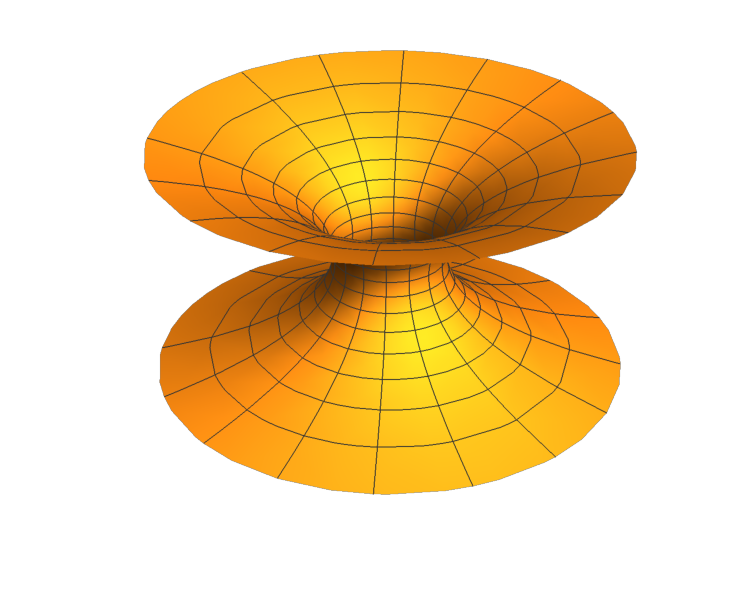
\includegraphics[scale=0.8]{images/catenoid.pdf}
\caption{Katenoida z implicitno enačbo~\eqref{eq:katenoida-implicitno}.}
\end{center}
\end{figure}

Opazimo, da je parametrizacija katenoide~\eqref{eq:katenoida} $2 \pi$-periodična glede na spremenljivko $u$. V Enneper-Weierstrassovo formulo helikatenoide~\eqref{eq:EP-helikatenoida} uvedimo novo spremenljivko $w = e^{i \zeta} \in \mathbb{C} \setminus \{0\}$ in vzemimo njen realni del. Računajmo
\begin{align*}
z(\zeta) &= (1,0,0) + \int_{0}^{\zeta} \left( \frac{1}{2} \left(\frac{1}{e^{i\xi}} - e^{i\xi} \right), \frac{i}{2} \left(\frac{1}{e^{i\xi}} + e^{i\xi} \right), 1 \right) (-i) d\xi \\
	&= (1,0,0) + \int_{1}^{w} \left( \frac{1}{2} \left(\frac{1}{\eta} - \eta \right), \frac{i}{2} \left(\frac{1}{\eta} + \eta \right), 1 \right) (-i) \frac{-i}{\eta} d\eta \\
	&= (1,0,0) - \int_{1}^{w} \left( \frac{1}{2} \left(\frac{1}{\eta} - \eta \right), \frac{i}{2} \left(\frac{1}{\eta} + \eta \right), 1 \right) \frac{d\eta}{\eta},
\end{align*}
kar nam da parametrizacijo katenoide $x \colon \mathbb{C} \setminus \{0\} \to \mathbb{R}^3$ z Enneper-Weierstrassovo formulo
\begin{equation}
x(w) = (1,0,0) - \Re \int_{1}^{w} \left( \frac{1}{2} \left(\frac{1}{\eta} - \eta \right), \frac{i}{2} \left(\frac{1}{\eta} + \eta \right), 1 \right) \frac{d\eta}{\eta}.
\end{equation}
Sledi, da je kompleksna Gaussova preslikava katenoide enaka $\mathfrak{g}(w) = w$ za $w \in \mathbb{C} \setminus \{0\}$, ki jo holomorfno razširimo do identične preslikave na $\mathbb{CP}^{1}$. Identiteta je preslikava stopnje $d=1$, zato iz teorije o Gaussovih preslikavah dobimo vrednost totalne Gaussove ukrivljenosti katenoide, ki znaša $-4 \pi$. Izkaže se, da je to edini primer iz družine pridruženih minimalnih ploskev k helikatenoidi s končno totalno Gaussovo ukrivljenostjo.

Katenoido je kot rotacijsko ploskev prvi opisal Leonhard Euler l.~1744. Dobro stoletje kasneje je P.~O.~Bonnet pokazal, da je to (razen ravnine) edina rotacijska minimalna ploskev v trirazsežnem prostoru. Ker je razmeroma enostavna in ima še več posebnih topoloških lastnosti, jo običajno spoznamo kot prvi primer pri študiju minimalnih ploskev.

%%%%%%%%%%%%%%%
% Helikoid
\subsubsection{Helikoid}
%
Negativno predznačeni imaginarni del helikatenoide imenujemo \emph{helikoid}. Natančneje, to je preslikava $y = -\Im z = \Re (iz) \colon \mathbb{R}^2 \to \mathbb{R}^3$ s konformno parametrizacijo
\begin{equation} \label{eq:helikoid}
y(u,v) = (\sin u \cdot \sinh v, -\cos u \cdot \sinh v, u).
\end{equation}
Helikoid je pridružena minimalna ploskev k helikatenoidu, ki ustreza parametrom $t = \frac{\pi}{2} + k \pi, \ k \in \mathbb{Z}$. (Res, $e^{it}z = iz$ natanko tedaj, ko je $t = \frac{\pi}{2} + 2k \pi, \ k \in \mathbb{Z}$. Z izbiro $t = \frac{\pi}{2} + k \pi, \ k \in \mathbb{Z}$, pa dobimo levi in desni helikoid.) Po definiciji sta katenoida in helikoid konjugirani minimalni ploskvi.

Geometrijsko helikoid dobimo na naslednji način: premico rotiramo okrog izbrane osi v $\mathbb{R}^3$ (tj.~v ravnini v $\mathbb{R}^3$) in jo hkrati premikamo vzdolž te osi (v pravokotni smeri glede na ravnino, v kateri premico rotiramo).

% slika helikoida
\begin{figure}[h!]
\begin{center}
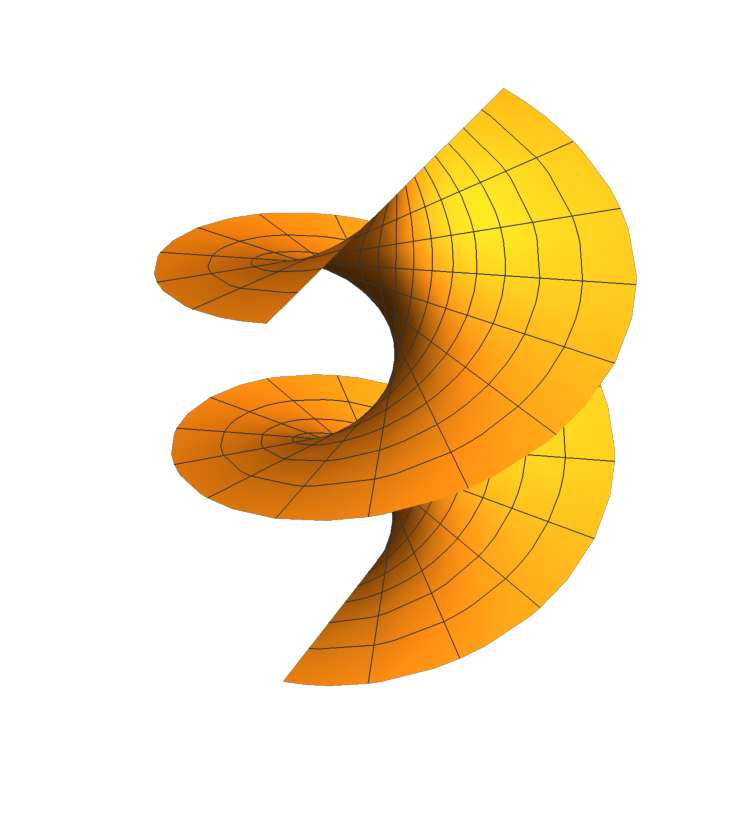
\includegraphics[scale=0.8]{images/helicoid.pdf}
\caption{Helikoid v $\mathbb{R}^3$ z $z$-osjo kot osjo rotacije.}
\end{center}
\end{figure}

Enneper-Weierstrassovo formulo helikoida dobimo iz izraza~\eqref{eq:EP-helikatenoida}:
\begin{align}
y(\zeta) &= \Re (iz(\zeta)) = \Re \left( (i,0,0) + \int_{0}^{\zeta} \left( \frac{1}{2} \left(\frac{1}{e^{i\xi}} - e^{i\xi} \right), \frac{i}{2} \left(\frac{1}{e^{i\xi}} + e^{i\xi} \right), 1 \right) (-i) i d\xi \right) \nonumber \\
	&= \Re \int_{0}^{\zeta} \left( \frac{1}{2} \left(\frac{1}{e^{i\xi}} - e^{i\xi} \right), \frac{i}{2} \left(\frac{1}{e^{i\xi}} + e^{i\xi} \right), 1 \right) d\xi, \quad \zeta \in \mathbb{C}.
\end{align}
Njegova kompleksna Gaussova preslikava je $\mathfrak{g}(\zeta) = e^{i\zeta}$, kar nam pove, da ima helikoid negativno neskončno totalno Gaussovo ukrivljenost; $TC(y) = -\infty$. 

O helikoidu sta prva pisala L.~Euler in J.~B.~Meusnier v 80.-ih letih 18.~stoletja, brez znanja o konjugiranih minimalnih ploskvah in povezavi s kompleksno analizo. Omenimo še dve zanimivi lastnosti obravnavane minimalne ploskve:
\begin{itemize}
\item Za vsako točko na helikoidu obstaja premica, ki leži na njem in gre skozi to točko.
\item Za vsako točko na helikoidu obstaja vijačnica, ki leži na njem in gre skozi to točko.
\end{itemize}
Prvo lastnost kot minimalni ploskvi v $\mathbb{R}^3$ premoreta le helikoid in ravnina, kar je l.~1842 dokazal E.~C.~Catalan. Druga lastnost namiguje na izvor imena -- helikoid spominja na latinsko besedo ``helix'', kar v slovenščini imenujemo vijačnica.

%%%%%%%%%%%%%%%
% Enneperjeva ploskev
\subsubsection{Enneperjeva ploskev}
%
Recimo, da poznamo par $(\mathfrak{g}, \phi_3)$, kjer sta $\mathfrak{g}(z) = z$ holomorfna preslikava in $\phi_3(z) = 2z$ holomorfna 1-forma ($z \in \mathbb{C}$).
Potem po zvezi~\eqref{eq:Weierstrass-podatki-Gauss3} vemo, da je meromorfna 1-forma $\Phi$ enaka
\begin{gather*}
\Phi = \left( \frac{1}{2} \left( \frac{1}{z} - z \right), \frac{i}{2} \left( \frac{1}{z} + z \right), 1 \right) \cdot 2z = \left( 1-z^2, i(1+z^2), 2z \right).
\end{gather*}
Enneper-Weierstrassova formula preslikave $x \colon \mathbb{C} \to \mathbb{R}^3$ se glasi
\begin{equation}
x(\zeta) = \Re \int_{0}^{\zeta} \left( 1-z^2, i(1+z^2), 2z \right) dz
\end{equation}
in določa minimalno ploskev, imenovano \emph{Enneperjeva ploskev}, ki jo je l.~1868 odkril A.~Enneper.

Če za $ u,v \in \mathbb{R}$ pišemo $\zeta = u + iv \in \mathbb{C}$ in po komponentah izračunamo realne dele zgornjega integrala, dobimo konformno parametrizacijo $x \colon \mathbb{R}^2 \to \mathbb{R}^3$,
\begin{equation}
x(u,v) = \left( \frac{u}{3} \left(3(1+v^2) - u^2 \right), \frac{v}{3} \left( v^2 - 3(1+u^2) \right), u^2 - v^2 \right).
\end{equation}

Iz izbire podatkov vemo, da je kompleksna Gaussova preslikava Enneperjeve ploskve enaka $\mathfrak{g}(z) = z$, zato ima le-ta podobno kot katenoida totalno Gaussovo ukrivljenost enako $-4 \pi$. Izkaže se, da sta to edini polni\footnote{Pot $\gamma \colon [0,a) \to M, \ a \in (0,+\infty]$, je \emph{divergentna}, če za vsako kompaktno podmnožico $K \subset M$ velja: $\gamma(t) \notin K$, ko $t \to a$. Če je vsaka divergentna pot v $M$ razreda $\mathcal{C}^{1}$ neskončne dolžine, Riemannovi mnogoterosti $M$ pravimo \emph{polna}.} neravni orientabilni minimalni ploskvi vloženi v $\mathbb{R}^3$, katerih totalna Gaussova ukrivljenost znaša $-4 \pi$. Poleg tega je Enneperjeva ploskev konjugirana sama sebi.

%%%%%%%%%%%%%%%%%%%%%%%%%%%%%%%%%%%%%%%%%%%%%%%%%%%%%%%%%%%%%%%%%%%%%%%%%%%%%
%%%%%%%%%%%%%%%%%%%%%%%%%%%%%%%%%%%%%%%%%%%%%%%%%%%%%%%%%%%%%%%%%%%%%%%%%%%%%
% Izreki o aproksimaciji in interpolaciji minimalnih ploskev
\section{Izreki o aproksimaciji in interpolaciji minimalnih ploskev}

Glavni cilj magistrske naloge so izreki o aproksimaciji in interpolaciji minimalnih ploskev, ki jih bomo predstavili v tem poglavju. Osnovna ideja so klasični aproksimacijski in interpolacijski izreki za holomorfne funkcije -- Rungejev, Bishop-Mergelyanov in Weierstrass-Florackov izrek (Izreki~\ref{izr:Runge}, \ref{izr:Bishop-Mergelyan}, \ref{izr:Weierstrass-Florack}), katere je potrebno ustrezno prilagoditi.

Osredotočili se bomo na povezane odprte Riemannove ploskve $M$ z izbrano fiksno strukturo kompleksne mnogoterosti, na katerih bomo definirali konformne minimalne imerzije $x \colon M \to \mathbb{R}^{n}$ oziroma holomorfne ničelne krivulje $z \colon M \to \mathbb{C}^{n}$ ($n \geq 3$).
V nekaterih primerih bomo za $M$ izbrali kompaktno Riemannovo ploskev z robom, natančneje, kompaktno domeno $M$ z gladkim robom $bM$, ki je podmnožica odprte Riemannove ploskve.

%%%%%%%%%%%%%%%%%%%%%%%%%%%%%%%%%%%%%%%%%%%%%%%%%%%%%%%%%%%%%%%%%%%%%%%%%%%%%
% Prostori preslikav in posplošene minimalne imerzije
\subsection{Prostori preslikav in posplošene minimalne imerzije}
%
Najprej definirajmo različne tipe konformnih minimalnih imerzij glede na njihovo sliko ter pripadajoče prostore preslikav.

% ravna, polna, neizrojena k.m.i.
\begin{definicija} \label{def:full-flat-nd}
Naj bo $M$ povezana odprta Riemannova ploskev ali kompaktna Riemannova ploskev z robom, na kateri je definirana povsod neničelna holomorfna 1-forma $\theta$. Konformno minimalno imerzijo $x \colon M \to \R^{n}$ imenujemo:
\begin{enumerate}
\item \emph{ravna}, če je slika $x(M)$ vsebovana v afini ravnini v $\R^{n}$; sicer pravimo, da je $x$ \emph{neravna};
\item \emph{polna}, če je preslikava $f = 2 \partial{x} / \theta \colon M \to \textbf{\textup{A}}_{*}^{n-1}$ polna, tj.~$\C$-linearna ogrinjača slike $f(M)$ je enaka $\C^{n}$;
\item \emph{neizrojena}, če slika $x(M)$ ni vsebovana v nobeni afini hiperravnini v $\R^{n}$. 
\end{enumerate}
\end{definicija}

% [CITIRAJ - Osserman, Lemma 12.4]
V dimenziji  $n=3$ za konformno minimalno imerzijo vsi zgornji pojmi sovpadajo. V višjih dimenzijah ($n \geq 4$) veljata implikaciji
\begin{gather} \label{implikacije:full-nd-nf}
\text{polna} \ \Rightarrow \ \text{neizrojena} \ \Rightarrow \ \text{neravna}.
\end{gather}
Obratne implikacije ne vejajo.

% prostori preslikav
Naj bosta $M$ in $X$ kompleksni mnogoterosti. Prostor holomorfnih preslikav $M \to X$ označimo z $\mathcal{O}(M,X)$.
Če je $K$ kompaktna podmnožica v $M$, množico preslikav $K \to X$ razreda $\mathcal{C}^{r}(M)$, ki so holomorfne v notranjosti $K^\circ \subset K$, označimo z $\mathcal{A}^{r}(K,X)$.
V primeru, ko je $X = \C$, ustrezna prostora označimo z $\mathcal{O}(M)$ oziroma $\mathcal{A}^{r}(K)$.

Naj bo $M$ odprta Riemannova ploskev in $n \geq 3$. Prostor konformnih minimalnih imerzij $M \to \R^{n}$ označimo s $\textup{CMI}(M, \R^{n})$, prostor holomorfnih ničelnih krivulj $M \to \C^{n}$ pa z $\textup{NC}(M, \C^{n})$. Oba prostora sta opremljena s kompaktno-odprto topologijo\footnote{Naj bosta $X$ in $Y$ topološka prostora ter $\mathcal{C}(X,Y)$ prostor zveznih preslikav med njima. Množica $\mathcal{V} = \{ f \in \mathcal{C}(X,Y); \ f(K) \subset U, \ K \subset X \ \text{kompaktna}, \ U \subset Y \ \text{odprta} \}$ tvori podbazo \emph{kompaktno-odprte topologije} na prostoru $\mathcal{C}(X,Y)$.}.
Nadalje $\textup{CMI}_{full}(M, \R^{n})$ in $\textup{CMI}_{nf}(M, \R^{n})$ označujeta prostora polnih oziroma neravnih konformnih minimalnih imerzij na povezanih komponentah $M$. Po zvezi~\eqref{implikacije:full-nd-nf} velja inkluzija 
\begin{gather*}
\textup{CMI}_{full}(M, \R^{n}) \subset \textup{CMI}_{nf}(M, \R^{n}).
\end{gather*}
%
Podobno je 
\begin{gather*}
\textup{NC}_{full}(M, \C^{n}) \subset \textup{NC}_{nf}(M, \C^{n})
\end{gather*} 
v primeru polnih ter neravnih holomorfnih ničelnih krivulj, saj analogna definicija k Definiciji~\ref{def:full-flat-nd} velja za holomorfne ničelne krivulje. Vsi ti prostori so odprti podprostori v $\textup{CMI}(M, \R^{n})$ oziroma $\textup{NC}(M, \C^{n})$.

Če je $M$ kompaktna Riemannova ploskev z nepraznim gladkim robom $bM$ in $r \in \N$, tedaj prostor konformnih minimalnih imerzij $M \to \R^{n}$ razreda $\mathcal{A}^{r}(M)$ označimo s $\textup{CMI}^{r}(M, \R^{n})$, prostor holomorfnih ničelnih krivulj $M \to \C^{n}$ razreda $\mathcal{A}^{r}(M)$ pa z $\textup{NC}^{r}(M, \C^{n})$.
Odprte podprostore polnih in neravnih preslikav tokrat označimo podobno kot prej; zanje velja
\begin{gather*}
\textup{CMI}_{full}^{r}(M, \R^{n}) \subset \textup{CMI}_{nf}^{r}(M, \R^{n}), \quad \textup{NC}_{full}^{r}(M, \C^{n}) \subset \textup{NC}_{nf}^{r}(M, \C^{n}).
\end{gather*}

\begin{opomba}
Imerzija $x \colon M \to \mathbb{R}^{n}$ razreda $\mathcal{A}^{r}(M)$ na kompaktni Riemannovi ploskvi z nepraznim gladkim robom $bM$ je element prostora $\textup{CMI}^{r}(M, \R^{n})$ natanko tedaj, ko je pripadajoča 1-forma $\partial x = (\partial x_{1}, \dots , \partial x_{n})$ holomorfna na $M^{\circ} = M \setminus bM$ in zadošča ničelnemu pogoju $(\partial{x_1})^2 + \cdots + (\partial{x_n})^2 = 0$.
\end{opomba}

% lema - neravna preslikava
\begin{lema} \label{lema:neravna f}
Naj bo $M$ povezana Riemannova ploskev in $\textbf{\textup{A}}_{*}$ punktirana ničelna kvadrika.
Holomorfna preslikava $f \colon M \to \textbf{\textup{A}}_{*}$ je neravna natanko tedaj, ko je linearna ogrinjača tangentnih prostorov 
$T_{f(p)} \textbf{\textup{A}} \subset T_{f(p)} \C^{n} \cong \mathbb{C}^{n}$ po vseh $p \in M$ enaka $\C^{n}$.
\end{lema}

\begin{dokaz}
Oglejmo si preslikavo 
$\Phi \colon \C^{n} \to \C$, definirano s predpisom $\Phi(z) = \sum_{j=1}^{n} z_{j}^{2}$.
Ničelno kvadriko~\eqref{ničelna-kvadrika} tedaj lahko zapišemo v obliki $\textbf{\textup{A}} = \Phi^{-1}( \{0 \} )$.
Njen tangentni prostor v točki $z = (z_{1}, \dots , z_{n}) \in \C^{n}$ je enak jedru diferenciala, ki kvadriko določa, zato je
\[ T_{z} \textbf{\textup{A}} = \ker (d \Phi_{z}) = \ker (z \mapsto \sum_{j=1}^{n} z_{j} dz_{j}). \]

Naj bosta vektorja $z, \ w \in \C_{*}^{n}$. Potem sta njuna tangentna prostora enaka, $ T_{z} \textbf{\textup{A}} = T_{w} \textbf{\textup{A}} $, natanko takrat, ko velja $z_{j} = \lambda w_{j}$ za vse $j = 1, \dots , n$ in nek $\lambda \in \C$, kar je ekvivalentno pogoju, da sta vektorja $z$ in $w$ kolinearna.

Po definiciji je preslikava $f$ neravna, če njena slika $f(M)$ ni vsebovana v nobeni afini kompleksni premici v $\C^{n}$. Skupaj z zgornjim je slednje ekvivalentno 
$ \mathcal{L}in \{T_{f(p)} \textbf{\textup{A}} ; \ p \in M \} = \C^{n}$, kar smo želeli dokazati.
\end{dokaz}

V aproksimacijskih in interpolacijskih izrekih bomo v dokazih namesto običajnih konformnih minimalnih imerzij in ničelnih krivulj operirali s splošnejšimi preslikavami, imenovanimi posplošene minimalne imerzije ter ničelne krivulje; naravno pa se bodo zaradi topoloških lastnosti množic, na katerih bomo preslikave aproksimirali, pojavile tudi množice iz naslednje definicije.
% dopustna množica
\begin{definicija} [Dopustna množica]
Naj bo $M$ gladka ploskev, $K$ končna unija paroma disjunktnih kompaktnih domen s kosoma zvezno odvedljivimi robovi v $M$ ter $E = S \setminus K^\circ$ unija končno mnogo paroma disjunktnih gladkih Jordanovih lokov in zaprtih Jordanovih krivulj, ki se dotikajo $K$ kvečjemu v svojih krajiščih in sekajo rob $K$ transverzalno. Kompaktno podmnožico v $M$ oblike $S = K \cup E$ imenujemo \emph{dopustna množica}.
\end{definicija}

% posplošena konformna minimalna imerzija
\begin{definicija} [Posplošena konformna minimalna imerzija]
Naj bo $S = K \cup E$ dopustna podmnožica Riemannove ploskve $M$ in $\theta$ povsod neničelna holomorfna 1-forma, definirana v okolici $S \subset M$.
Naj bosta $n \geq 3$ in $r \in \N$. \emph{Posplošena konformna minimalna imerzija} $S \to \R^{n}$ razreda $\mathcal{C}^{r}$ je par $(x, f \theta)$, kjer je $x \colon S \to \R^{n}$ preslikava razreda  $\mathcal{C}^{r}$, njena zožitev na $S^\circ = K^\circ$ je konformna minimalna imerzija in preslikava $f \in \mathcal{A}^{r-1}(S, \textbf{\textup{A}}_{*})$ zadošča naslednjima pogojema:
\begin{enumerate}
\item na množici $K$ velja $f \theta = 2 \partial x$;
\item za vsako gladko pot $\alpha$ v $M$, ki parametrizira povezano komponento množice $E = \overline{S \setminus K}$, velja $ \Re(\alpha^{*}(f \theta)) = \alpha^{*}(dx) = d(x \circ \alpha)$.
\end{enumerate}
%
Posplošena konformna minimalna imerzija $(x, f \theta)$ je \emph{neravna} oziroma \emph{polna} natanko tedaj, ko je preslikava $f \in \mathcal{A}^{r-1}(S, \textbf{\textup{A}}_{*})$ neravna oziroma polna na vsaki relativno odprti podmnožici $S$.
\end{definicija}

Prostor posplošenih konformnih minimalnih imerzij $S \to \R^{n}$ razreda $\mathcal{C}^{r}$ označimo z $\textup{GCMI}^{r}(S, \R^{n})$. Analogno kot v primeru konformnih minimalnih imerzij velja 
\begin{gather*}
\textup{GCMI}_{full}^{r}(S, \R^{n}) \subset \textup{GCMI}_{nf}^{r}(S, \R^{n}) \subset \textup{GCMI}^{r}(S, \R^{n}).
\end{gather*}

\begin{opomba}
Spomnimo se diferenciala in konjugiranega diferenciala v kompleksnem. Zanju velja $d + i d^{c} = 2 \partial$ oziroma drugače, $\Re(2 \partial x) = dx$.
Prvi pogoj iz definicije posplošene konformne minimalne imerzije pravi $f \theta = 2 \partial x$, od koder sledi $\Re(f \theta) = \Re(2 \partial x) = dx$. Zato je drugi pogoj iz zgornje definicije skladen s prvim.
\end{opomba}

Tudi za posplošene konformne minimalne imerzije velja Enneper-Weierstrassova formula.
Naj bo $S$ povezana dopustna množica in $(x, f \theta) \in \textup{GCMI}^{r}(S, \R^{n})$. Za poljubno točko $p_{0} \in S$ in poznano preslikavo $f$ lahko posplošeno konformno minimalno imerzijo $x \colon S \to \R^{n}$ konstruiramo s formulo
\begin{align} \label{eq:EW-gcmi}
x(p) = x(p_{0}) + \Re \int_{p_0}^{p} f \theta, \quad p \in S.
\end{align} 
Obratno, če za preslikavo $f \in \mathcal{A}^{r-1}(S, \textbf{\textup{A}}_{*})$ velja $ \Re \int_{C} f \theta = 0$ za vsako sklenjeno krivuljo $C$ v $S$, potem le-ta določa posplošeno konformno minimalno imerzijo, dano z Enneper-Weierstrassovo formulo~\eqref{eq:EW-gcmi}.

% posplošena ničelna krivulja
\begin{definicija} [Posplošena ničelna krivulja]
Naj bo $S = K \cup E$ dopustna podmnožica Riemannove ploskve $M$ in $\theta$ povsod neničelna holomorfna 1-forma, definirana v okolici $S \subset M$.
Naj bosta $n \geq 3$ in $r \in \N$. \emph{Posplošena ničelna krivulja} $S \to \C^{n}$ razreda $\mathcal{C}^{r}$ je par $(z, f \theta)$, kjer preslikavi $z \in \mathcal{A}^{r}(S, \C^{n})$ in $f \in \mathcal{A}^{r-1}(S, \textbf{\textup{A}}_{*})$ zadoščata naslednjima pogojema:
\begin{enumerate}
\item na množici $K$ velja $f \theta = dz = \partial z$;
\item za vsako gladko pot $\alpha$ v $M$, ki parametrizira povezano komponento množice $E = \overline{S \setminus K}$ velja $ \alpha^{*}(f \theta) = \alpha^{*}(dz) = d(z \circ \alpha)$.
\end{enumerate}
%
Posplošena ničelna krivulja $(z, f \theta)$ je \emph{neravna} oziroma \emph{polna} natanko tedaj, ko je preslikava $f \in \mathcal{A}^{r-1}(S, \textbf{\textup{A}}_{*})$ neravna oziroma polna na vsaki relativno odprti podmnožici $S$.
\end{definicija}

Prostori neravnih, polnih in posplošenih ničelnih krivulj ustrezajo verigi inkluzij
\begin{gather*}
\textup{GNC}_{full}^{r}(S, \C^{n}) \subset \textup{GNC}_{nf}^{r}(S, \C^{n}) \subset \textup{GNC}^{r}(S, \C^{n}).
\end{gather*}

\begin{opomba}
Iz prvega pogoja v definiciji posplošene ničelne krivulje sledi, da je zožitev $z \colon K^{\circ} \to \mathbb{C}^{n}$ holomorfna ničelna krivulja.
\end{opomba}

Za povezano dopustno množico $S$, par $(z, f \theta) \in \textup{GNC}^{r}(S, \C^{n})$, znano preslikavo $f$ in poljubno točko $p_{0} \in S$ posplošeno ničelno krivuljo $z \colon S \to \C^{n}$ konstruiramo s pomočjo Enneper-Weierstrassove formule
\begin{align} \label{eq:EW-gnc}
z(p) = z(p_{0}) + \int_{p_0}^{p} f \theta, \quad p \in S.
\end{align} 
Velja tudi obrat; preslikava $f \in \mathcal{A}^{r-1}(S, \textbf{\textup{A}}_{*})$, ki zadošča $\int_{C} f \theta = 0$ za vsako sklenjeno krivuljo $C$ v $S$, določa posplošeno ničelno krivuljo, dano z Enneper-Weierstrassovo formulo~\eqref{eq:EW-gnc}.

%%%%%%%%%%%%%%%%%%%%%%%%%%%%%%%%%%%%%%%%%%%%%%%%%%%%%%%%%%%%%%%%%%%%%%%%%%%%%
% Periodno dominantni spreji
\subsection{Periodno dominantni spreji}
%
V tem razdelku bomo definirali pojem periodno dominantnega spreja holomorfnih preslikav v punktirano ničelno kvadriko. Glavni rezultat bo lema, ki opisuje neravne holomorfne preslikave iz dopustne množice v punktirano ničelno kvadriko -- izkaže se, da je vsaka taka preslikava jedro periodno dominantnega spreja. Lema je pomembna pri aproksimaciji konformnih minimalnih imerzij. Natančneje, namesto imerzij bomo najprej aproksimirali periodno dominantne spreje in s tem dobili nove, bližnje preslikave z želenimi topološkimi lastnostmi, nato pa zanje uporabili Enneper-Weierstrassovo formulo ter končno dobili bližnje konformne minimalne imerzije.

\begin{definicija} [Periodna preslikava]
Naj bo $M$ povezana odprta Riemannova ploskev in $\theta$ fiksna povsod neničelna holomorfna 1-forma na $M$. Naj bo $\mathcal{C} = \{C_1, \dots , C_{l} \}$ družina gladkih orientiranih vloženih lokov in zaprtih Jordanovih krivulj v $M$ ter $C = \cup_{i=1}^{l} C_{i}$.
Družini $\mathcal{C}$ in številu $n \in \N$ priredimo \emph{periodno preslikavo}
\begin{gather}
\mathcal{P} = (\mathcal{P}_1, \dots , \mathcal{P}_{l}) \colon \mathcal{C}(C, \C^{n}) \to (\C^{n})^{l}, \nonumber \\
\mathcal{P}_{i}(f) = \int_{C_{i}} f \theta, \quad i=1, \dots , l.
\end{gather}
Tu je $f \in \mathcal{C}(C, \C^{n})$ in $\mathcal{P}_{i}(f) \in \C^{n}$.
\end{definicija}

% lema - periodno dominantni sprej 
\begin{lema} \label{lema:P-D-sprej}
Naj bo $M$ odprta Riemannova ploskev in $S = K \cup E$ njena dopustna podmnožica. Naj bo $\mathcal{C} = \{C_1, \dots , C_{l} \}$ taka družina gladkih orientiranih Jordanovih krivulj in lokov v $S$, da je unija $C = \cup_{i=1}^{l} C_{i}$ Rungejeva v $S$.
Naj za neko število $r \in \Z_{+}$ preslikava $f \colon S \to \textbf{\textup{A}}_{*}$ pripada razredu $\mathcal{A}^{r}$.
Nadalje predpostavimo, da vsaka krivulja $C_{i} \in \mathcal{C}$ vsebuje netrivialen lok $I_{i} \subset C_{i}$, disjunkten z $\cup_{i \neq j}C_{j}$, preslikava $f \colon I_{i} \to \textbf{\textup{A}}_{*}$ pa je neravna.

Potem obstaja odprta okolica $U \subset \C^{ln}$ točke $0$ in preslikava $\Phi_{f} \in \mathcal{A}^{r} (S \times U, \textbf{\textup{A}}_{*})$, tako da velja
$\Phi_{f}(\cdot, 0) = f$ in je preslikava
\begin{gather} \label{PD-lastnost}
	 \frac{\partial}{\partial t} \Big|_{t=0} \mathcal{P}(\Phi_{f}(\cdot, t)) \colon (\C^{n})^{l} \to (\C^{n})^{l} \ \text{izomorfizem.}
\end{gather}

Nadalje, za končno podmnožico $P \subset S$ lahko preslikavo $\Phi_{f}$ izberemo tako, da se za $t \in U$ preslikave $\Phi_{f}(\cdot, t) \colon S \to\textbf{\textup{A}}_{*}$ ujemajo z $f$ v vsaki točki $P \setminus S^\circ$, v točkah $P \cap S^\circ$ pa se z $f$ ujemajo do danega končnega reda.

Za vsako preslikavo $f_{0} \in \mathcal{A}^{r}(S, \textbf{\textup{A}}_{*})$, ki zadošča zgornjim predpostavkam, obstaja okolica $\Omega \subset \mathcal{A}^{r}(S, \textbf{\textup{A}}_{*})$ in holomorfna preslikava $f \mapsto \Phi_{f}$, $f \in \Omega$, z zgornjimi lastnostmi.
\end{lema}

\begin{definicija} [Periodno dominantni sprej]
Preslikavo $\Phi_{f}$, ki ustreza Lemi~\ref{lema:P-D-sprej} imenujemo \emph{periodno dominantni sprej} preslikav $S \to \textbf{\textup{A}}_{*}$ za družino krivulj $\mathcal{C}$ z \emph{jedrom} $\Phi_{f}(\cdot, 0) = f$. Lastnosti~\eqref{PD-lastnost} pravimo \emph{periodno dominantna lastnost}.
\end{definicija}

%%%%% dokaz leme
\begin{dokaz}
Prvi del leme bomo dokazali tako, da bomo konstruirali periodno dominantni sprej. Potrebovali bomo Lemo~\ref{lema:neravna f}, Bishop-Mergelyanov izrek o aproksimaciji~\ref{izr:Bishop-Mergelyan} in pojem toka vektorskega polja.
Zaradi enostavnosti postavimo $r=0$ (za $r>0$ dokaz poteka analogno).

Po predpostavki je za vse $i \in \{ 1, \dots, l \}$ lok $I_{i} \subset C_{i} \in \mathcal{C}$ netrivialen, za katerega velja $I_{i} \cap (\cup_{i \neq j} C_{j}) = \emptyset$ in je zožitev preslikave $f|_{I_{i}}$ neravna. Po Lemi~\ref{lema:neravna f} zato obstajajo točke $p_{i,j} \in I_{i}$ in taka holomorfna vektorska polja $V_{i,j}$ na $\C^{n}$, $j \in \{1, \dots, n \}$, ki so tangentna na $\textbf{\textup{A}}$, da je $\mathcal{L}in \{ V_{i,j}(f(p_{i,j})) ; \ j = 1, \dots, n \} = \C^{n}$ za vse $i$.

Za $k = 1, \dots , l$ označimo $t_{k} = (t_{k,1}, \dots, t_{k,n}) \in \C^{n}$ in $t = (t_{1}, \dots, t_{l}) \in \C^{nl}$. Naj $\Phi_{t}^{i,j}$ označuje tok vektorskega polja $V_{i,j}$, definiran za majhne $t$. (Seveda so tokovi holomorfne preslikave.)
Okolico $U_{0} \subset \C^{nl}$ točke $0$ izberimo tako, da za vse $t \in U_{0}$ in $p \in S$ predpis
\begin{gather} \label{predpis-tokovi}
(p, t) \mapsto \Phi_{t_{1,1}}^{1,1} \circ \cdots \circ \Phi_{t_{1,n}}^{1,n} \circ \Phi_{t_{2,1}}^{2,1} \circ \cdots \circ \Phi_{t_{l,n}}^{l,n} (f(p))
\end{gather}
podaja dobro definirano preslikavo $S \times U_{0} \to \textbf{\textup{A}}_{*}$.
Sedaj za vse pare $(i,j)$ izberimo gladke preslikave $g_{i,j} \colon C \to \C$, pri čemer je nosilec od $g_{i,j}$ vsebovan v majhnem delu loka $I_{i}$ okrog točke $p_{i,j} \in I_{i}$.
Modificirana preslikava~\eqref{predpis-tokovi}, $\Phi \colon C \times U_{1} \to \textbf{\textup{A}}_{*}$,
\begin{gather} \label{predpis-Phi}
\Phi(p,t) = \Phi_{g_{1,1}(p)t_{1,1}}^{1,1} \circ \cdots \circ \Phi_{g_{1,n}(p)t_{1,n}}^{1,n} \circ \Phi_{g_{2,1}(p)t_{2,1}}^{2,1} \circ \cdots \circ \Phi_{g_{l,n}(p)t_{l,n}}^{l,n} (f(p)),
\end{gather}
kjer je $U_{1} \subset \C^{nl}$ primerno majhna okolica točke $0$, je tedaj dobro definirana, za vse $p \in C$ pa je preslikava $\Phi(p, \cdot) \colon U_{1} \to \textbf{\textup{A}}_{*}$ holomorfna. Po lastnostih toka vektorskega polja sledi še $\Phi(p,0) = f(p)$ za vse $p \in C$ in
\begin{equation} \label{dPhi/dt}
\frac{\partial \Phi(p,t)}{\partial t_{m,j}} \Big|_{t=0} = g_{m,j}(p) \cdot V_{m,j}(f(p)).
\end{equation}

Naj bo $\mathcal{P} = (\mathcal{P}_{1}, \dots, \mathcal{P}_{l})$ periodna preslikava, prirejena družini krivulj $\mathcal{C}$. Z uporabo enakosti~\eqref{dPhi/dt} dobimo za vse indekse $i, m \in \{1, \dots, l \}$ in $j \in \{1, \dots, n \}$
\begin{gather} \label{eq:dP/dt}
\frac{\partial \mathcal{P}_{i}(\Phi(\cdot, t))}{\partial t_{m,j}} \Big|_{t=0} = \frac{\partial}{\partial t_{m,j}} \Big|_{t=0} \int_{C_{i}} \Phi(\cdot, t) \cdot \theta = \int_{C_{i}} g_{m,j} \cdot (V_{m,j} \circ f) \cdot \theta \in \C^{n}.
\end{gather}
Matrika diferencialov~\eqref{PD-lastnost} iz leme je sestavljena iz blokov velikosti $n \times n$, ki pripadajo indeksom $i, m \in \{1, \dots, l \}$. Z ustrezno izbiro preslikav $g_{i,j}$, opisanih zgoraj, lahko dosežemo, da je matrika bločno diagonalna z obrnljivimi bloki na diagonali. (To pomeni, da so vektorji~\eqref{eq:dP/dt} blizu vektorjem $V_{i,j}(f(p_{i,j}))$ za $i = m$, medtem ko so za $i \neq m$ vektorji~\eqref{eq:dP/dt} ničelni.) S tem postane celotna matrika obrnljiva.

V naslednjem koraku bomo modificirali še preslikavo $\Phi$, kar nam bo dalo iskani periodno dominantni sprej.
Preslikave $g_{i,j}$ so definirane na množici $C$, ki je po predpostavki Rungejeva v $S$. Bishop-Mergelyanov izrek o aproksimaciji pove, da vsako funkcijo $g_{i,j}$ lahko enakomerno na $C$ aproksimiramo s holomorfnimi funkcijami $\tilde{g}_{i,j}$ v okolici $S$.

Definirajmo preslikavo $\Phi_{f} \colon S \times U \to \textbf{\textup{A}}_{*}$ tako, da v predpisu~\eqref{predpis-Phi} nadomestimo $g_{i,j}$ z novimi preslikavami $\tilde{g}_{i,j}$ in je $U \subset U_{1} \subset \C^{nl}$ ustrezno majhna okolica točke $0 \in \mathbb{C}^{nl}$. Po konstrukciji takšna preslikava $\Phi_{f}$ zadošča sklepom leme, zato je periodno dominantni sprej, ki smo ga iskali.

% interpolacijski del leme
Sedaj poglejmo še interpolacijski del leme. Naj bo $P \subset S$ končna podmnožica in $q \in \mathbb{N}$ izbrano fiksno število. Vzemimo holomorfno funkcijo $h \colon S \to \mathbb{C}$, ki ima ničle natanko v točkah množice $P$, le-te pa so reda $q+1$. Kot prej obstajajo točke $p_{i,j} \in I_{i} \setminus P$, holomorfna vektorska polja $V_{i,j} \in \mathbb{C}^{n}$ ter gladke preslikave $g_{i,j}$ s kompaktnimi nosilci okrog točk $p_{i,j}$. V predpisu~\eqref{predpis-Phi} najprej nadomestimo $g_{i,j}$ s preslikavami $h \cdot g_{i,j}$, da dobimo preslikavo $\Phi$, ki zadošča analogu k~\eqref{eq:dP/dt}. Nato preslikave $g_{i,j}$ aproksimiramo z $\tilde{g}_{i,j} \in \mathcal{O}(S)$ ter v predpis~\eqref{predpis-Phi} vstavimo produkte $h \cdot \tilde{g}_{i,j}$ -- nova preslikava $\Phi_{f}$ definira periodno dominantni sprej, ki dodatno zadošča interpolacijskim zahtevam.
Res, preslikava $(p,t) \mapsto \Phi_{h(p) \tilde{g}_{m,j}(p) t}^{m,j} (f(p))$ se z $f$ ujema v točkah množice $P$, v točkah $p \in P \cap S^{\circ}$ pa se ujemata do reda $q$. (To vidimo tako, da tok vektorskega polja zapišemo s Taylorjevim razvojem do 2.~reda in upoštevamo stopnje ničel funkcije $h$ v točkah $p \in P$.) Zato enako velja tudi za njihov kompozitum.
% Zadnji del - CITIRAJ VIR 12, Lemma 2.2

Za zadnji del leme opazimo naslednje: če je preslikava $f_{0} \in \mathcal{A}^{r}(S, \textbf{\textup{A}}_{*})$ dana, potem lahko za vse preslikave $f$ iz okolice $\Omega \subset \mathcal{A}^{r}(S, \textbf{\textup{A}}_{*})$ za $f_{0}$ pri konstrukciji periodno dominantnih sprejev uporabimo iste aproksimacijske preslikave $\tilde{g}_{i,j}$.
\end{dokaz}
%%%%% konec dokaza

% globalno def. PDS
\begin{opomba} \label{op:PDS-globalno}
Če v zgornjem dokazu izberemo polna holomorfna vektorska polja $V_{i,j} \in \mathbb{C}^{n}$, namesto lokalnega konstruiramo globalno definiran periodno dominantni sprej $\Phi_{f} \colon S \times \mathbb{C}^{n} \to \textbf{\textup{A}}_{*}$.
\end{opomba}

%%%%%%%%%%%%%%%%%%%%%%%%%%%%%%%%%%%%%%%%%%%%%%%%%%%%%%%%%%%%%%%%%%%%%%%%%%%%%
% Aproksimacija in interpolacija preslikav v punktirano ničelno kvadriko
\subsection{Aproksimacija in interpolacija preslikav v punktirano ničelno kvadriko}
%
% CITIRAJ [Theorem 1.13.1 & 1.13.3, Theorem 1.12.11: Minimal surfaces from a complex...]
Prvi rezultat o aproksimaciji in interpolaciji je Lema~\ref{lema:aproks&interp-A*}, ki opisuje preslikave iz povezane dopustne podmnožice odprte Riemannove ploskve v punktirano ničelno kvadriko $\textbf{\textup{A}}_{*} \subset \mathbb{C}^{n}$.
V dokazu leme bomo potrebovali pojem Oka mnogoterosti, katerega definicija sledi, z lastnostjo povezanih dopustnih množic, ki premorejo končno Rungejevo bazo homologije, pa bomo lahko uporabili rezultat prejšnjega razdelka o periodno dominantih sprejih (Lema~\ref{lema:P-D-sprej}).
Za iskanje bližnjih preslikav tistih, ki nastopajo v periodno dominantnem spreju, se bomo sklicali na različice Izrekov~\ref{izr:Runge},~\ref{izr:Bishop-Mergelyan} in~\ref{izr:Weierstrass-Florack}, tokrat za preslikave v (Oka) mnogoterosti, %(citiraj izreka 1.13.1, 1.13.3)
ter preslikave, definirane na dopustnih množicah. %(citiraj izrek 1.12.11)

% Oka mnogoterost
\begin{definicija} [Oka mnogoterost]
Naj bo $X$ kompleksna mnogoterost in $n \in \mathbb{N}$. Če za poljubno kompaktno konveksno množico $K \subset \mathbb{C}^{n}$ vsako holomorfno preslikavo $f \colon U \to X$, kjer je $U$ okolica $K$, lahko aproksimiramo enakomerno na $K$ s celimi preslikavami $F \colon \mathbb{C}^{n} \to X$, potem mnogoterosti $X$ pravimo \emph{Oka mnogoterost}.
\end{definicija}

% CITIRAJ [Definition 1.13.7, Minimal surfaces from a complex analytic viewpoint (fleksibilna mnt.)] & [Stein mnf's and holomorphic mappings, Forstneric: Proposition 5.6.22]
\begin{primer} [$\textbf{\textup{A}}_{*}$ je Oka mnogoterost] \label{primer-oka}
Naj bo $z = (z_{1}, \dots , z_{n}) \in \mathbb{C}^{n}$ in $n \geq 2$. Tedaj  homogen kvadratni polinom $p(z) = z_{1}^{2} + \cdots + z_{n}^{2}$ določa ničelno kvadriko $\textbf{\textup{A}} = \{z ; \ p(z)=0 \} \subset \mathbb{C}^{n}$.
Za indekse $1 \leq i \neq j \leq n$ definirajmo holomorfna vektorska polja na $ \textbf{\textup{A}}_{*} = \textbf{\textup{A}} \setminus \{ 0 \}$ s predpisi
\begin{gather*}
V_{ij} = z_{i} \frac{\partial}{\partial z_{j}} - z_{j} \frac{\partial}{\partial z_{i}}.
\end{gather*}
Očitno so vektorska polja $\mathbb{C}$-linearna in polna, tangentna na punktirano ničelno kvadriko $\textbf{\textup{A}}_{*}$ in $\mathcal{L}in \{ V_{ij}(x) ; \ x \in \textbf{\textup{A}}_{*} \} = T_{x}\textbf{\textup{A}}_{*}$. Po definiciji je zato kompleksna mnogoterost $\textbf{\textup{A}}_{*}$ \emph{fleksibilna mnogoterost}, kar pomeni, da je tudi Oka mnogoterost.
\end{primer}

% CITIRAJ [Lemma 1.12.10]
Naslednja lema, ki jo navajamo brez dokaza, trdi, da ima povezana dopustna množica posebno bazo homologije. Ideja dokaza, to je konstrukcija Jordanovih krivulj, ki tvorijo homološko bazo, bo za nas pomembna v nadaljevanju. Natančneje, pri aproksimaciji in interpolaciji minimalnih ploskev bomo interpolacijskim pogojem med drugim zadostili s kontroliranjem integralov po teh krivuljah.

\begin{lema} [Rungejeva baza homologije povezane dopustne množice] \label{lema:Runge-hom-baza}
Naj bo $S$ povezana dopustna množica. Obstaja baza homologije $\mathcal{C} = \{ C_{1}, \dots , C_{l} \}$ za $S$, sestavljena iz takih zaprtih odsekoma gladkih Jordanovih krivulj v $S$, da je unija $C = \cup_{i=1}^{l} C_{i}$ povezana in Rungejeva v vsaki regularni okolici $S_{\varepsilon}$ množice $S$, vsaka krivulja $C_{i}$ pa vsebuje netrivialen lok $I_{i}$, za katerega je $I_{i} \cap (\cup_{j \neq i} C_{j}) = \emptyset$.
Prva homološka grupa povezane dopustne množice $S$ je končno generirana: $H_{1}(S, \mathbb{Z}) \cong \mathbb{Z}^{l}$.
\end{lema}

Za $\varepsilon > 0$ je \emph{regularna okolica} dopustne množice $S \subset M$ enaka
\begin{gather}
S_{\varepsilon} = \{ x \in M; \ d(x,S) < \varepsilon \}.
\end{gather}
Množica $S_{\varepsilon}$ je odprta okolica za $S$, slednja nima lukenj v $S_{\varepsilon}$, zato je $S$ Rungejeva podmnožica svoje regularne okolice.

Sedaj imamo pripravljena vsa orodja za razumevanje aproksimacije in interpolacije preslikav v punktirano ničelno kvadriko.

% lema - aproksimacija in interpolacija preslikav v A*
\begin{lema} \label{lema:aproks&interp-A*}
Naj bo $M$ povezana odprta Riemannova ploskev in $S = K \cup E$ njena Rungejeva dopustna podmnožica.
Izberimo tako družino gladkih orientiranih Jordanovih krivulj in lokov v $S$, $\mathcal{C} = \{ C_{1}, \dots , C_{l} \}$, da je unija $C = \cup_{i=1}^{l} C_{i}$ Rungejeva v $M$, vsaka krivulja $C_{i}$ pa vsebuje netrivialen lok $I_{i}$, za katerega je $I_{i} \cap (\cup_{j \neq i} C_{j}) = \emptyset$.
Naj bo $\mathcal{P}$ periodno dominantni sprej, ki pripada družini krivulj $\mathcal{C}$, $A = \{ a_{1}, \dots , a_{m} \} \subset S$ končna množica točk in $r \geq 1$.
Tedaj lahko vsako preslikavo $f \in \mathcal{A}^{r}(S, \textbf{\textup{A}}_{*})$ aproksimiramo v $\mathcal{C}^{r}(S)$ s polnimi holomorfnimi preslikavami $F \in \mathcal{O}(M,\textbf{\textup{A}}_{*})$, pri čemer velja naslednje:
\begin{enumerate}
\item $\mathcal{P}(F) = \mathcal{P}(f)$;
\item preslikavi $F$ in $f$ se ujemata v točkah množice $A$, v točkah množice $A \cap S^{\circ}$ pa se ujemata do danega končnega reda.
\end{enumerate}
\end{lema}

%%%%% dokaz leme
\begin{dokaz}
Lemo bomo dokazali v dveh korakih. Najprej bomo $f \in \mathcal{A}^{r}(S, \textbf{\textup{A}}_{*})$ aproksimirali in interpolirali s polno preslikavo $g \in \mathcal{A}^{r}(S, \textbf{\textup{A}}_{*})$, za katero je $\mathcal{P}(f) = \mathcal{P}(g)$.
V drugem delu bomo s pomočjo Leme~\ref{lema:P-D-sprej} konstruirali periodno dominantni sprej preslikav iz množice $\mathcal{A}^{r}(S, \textbf{\textup{A}}_{*})$ z jedrom $g$. Nato bomo z izrekoma Mergelyana in Rungeja o aproksimaciji in interpolaciji preslikav iz odprtih Riemannovih ploskev v $\textbf{\textup{A}}_{*}$ periodno dominantni sprej aproksimirali in interpolirali s sprejem iz $\mathcal{O}(M, \textbf{\textup{A}}_{*})$, ki nam bo dal preslikavo $F   \in \mathcal{O}(M, \textbf{\textup{A}}_{*})$, ustrezno zaključkom leme. \newline

% 1. korak
1.~korak: Naj bo $S = K$ povezana kompaktna množica. (Za splošnejšo dopustno množico $S = K \cup E$ je korak enak, le da ga ponovimo na vsaki povezani komponenti $K$, na $E$ pa polno preslikavo dobimo z manjšo gladko deformacijo preslikave $f$.)
Predpostavimo, da $f$ ni polna. Sicer nadaljujemo z drugim korakom.
Označimo $\Sigma(f) = \mathcal{L}in (f(K)) \subset \mathbb{C}^{n}$, ki je po predpostavki pravi podprostor v $\mathbb{C}^{n}$.
Izberimo točke $x_{1}, \dots , x_{j} \in K \setminus A$ tako, da je $\Sigma(f) = \mathcal{L}in \{ f(x_{1}), \dots , f(x_{j}) \}$.
Ker je $\dim \Sigma(f) \leq n-1$, obstaja holomorfno vektorsko polje $V$ na $\mathbb{C}^{n}$ tangentno na $\textbf{\textup{A}}$, za katerega velja $V(f(x_0)) \notin \Sigma(f)$ za neko točko $x_0 \in K \setminus (A \cup \{ x_{1}, \dots , x_{j} \})$.

Naj bo $t \mapsto \Phi_{t}(z)$ tok vektorskega polja $V$ in $s \in \mathbb{N}$. 
Izberimo holomorfno funkcijo $h \colon K \to \mathbb{C}$ z lastnostmi:
\begin{itemize}
\item $h(x_{1}) = \dots = h(x_{j}) = 0$;
\item $h$ ima ničle reda $s$ v točkah množice $A$;
\item $h(x_0) = 1$.
\end{itemize}
Za poljubno funkcijo $\eta \in \mathcal{A}^{r}(K)$, ki je blizu ničelne funkcije, definirajmo preslikavo $\Psi (\eta) \in \mathcal{A}^{r}(K, \textbf{\textup{A}}_{*})$ s predpisom
\begin{gather}
\Psi (\eta)(x) = \Phi _{\eta(x) h(x)} f(x), \quad x \in K.
\end{gather}
Obstaja taka nekonstantna funkcija $\xi \in \mathcal{A}^{r}(K)$, ki je poljubno blizu ničelne funkcije, da je
\begin{gather*}
\mathcal{P}(\Psi (\xi)) = \mathcal{P}(\Psi(0)) = \mathcal{P}(f).
\end{gather*}
Označimo $g = \Psi(\xi)$. Velja naslednje:
\begin{itemize}
\item $g(x_{i}) = \Psi(\xi)(x_{i}) = \Phi_{\xi(x_{i}) h(x_{i})} f(x_{i}) = f(x_{i})$ za $i \in \{1, \dots , j \}$, saj je $h(x_{i})=0$. Sledi 
	$\Sigma(f) \subset \Sigma(g)$.
\item Produkt $\xi h$ je nekonstanten na kompaktu $K$, zato lahko dosežemo $\xi (x_0) \neq 0$ in $h(x_0) \approx 1.$ Potem velja
	$g(x_0) = \Psi(\xi)(x_0) = \Phi_{\xi(x_0) h(x_0)} f(x_0) \approx f(x_0) + \xi(x_0) h(x_0) V(f(x_0)) \notin \Sigma(f)$ po izboru $V$ in $x_0$.
\item Ker ima $h$ ničle reda $s$ v točkah množice $A$, s podobnim razvojem kot v prejšnji točki vidimo, da je $g|_{A} = f|_{A}$, v točkah $A \cap S^{\circ}$ pa se funkciji ujemata do reda $s$.
\end{itemize}
Induktivno nadaljujemo postopek tako, da višamo razsežnost prostora $\Sigma(f)$. Ko je $\dim \Sigma(f) = n-1$, dobimo polno preslikavo $g \in \mathcal{A}^{r}(S, \textbf{\textup{A}}_{*})$, ki aproksimira in interpolira $f$ ter zadošča pogoju $\mathcal{P}(g) = \mathcal{P}(f)$. \newline

% 2. korak
2.~korak: Novo preslikavo $g$ iz 1.~koraka preimenujmo v $f$. Ta je polna in zato neravna.
Lema~\ref{lema:Runge-hom-baza} pove, da povezana dopustna množica $S$ premore končno bazo homologije, sestavljeno iz posebnih Jordanovih krivulj. Skupaj z Lemo~\ref{lema:P-D-sprej} in Opombo~\ref{op:PDS-globalno} tako dobimo periodno dominantni sprej $\Phi_{f} \colon S \times \mathbb{C}^{N} \to \textbf{\textup{A}}_{*}$ z jedrom $f$.

Po predpostavki je $S$ Rungejeva podmnožica $M$, iz Primera~\ref{primer-oka} pa vemo, da je kvadrika $\textbf{\textup{A}}_{*}$ Oka mnogoterost.
Izreka Rungeja in Mergelyana o aproksimaciji in interpolaciji preslikav v Oka mnogoterosti zagotavljata obstoj holomorfne preslikave $\tilde{f} \colon M \to \textbf{\textup{A}}_{*}$, ki v $\mathcal{C}^{r}(S)$ aproksimira preslikavo $f$, $\tilde{f}$ se z $f$ ujema v točkah množice $A$, v točkah preseka $A \cap S^{\circ}$ pa se ujemata do danega končnega reda.

Podobno kot v dokazu Leme~\ref{lema:P-D-sprej} lahko po Mergelyanovem izreku o aproksimaciji na dopustnih množicah funkcije $g_{i,j} \in \mathcal{A}^{r}(S)$ iz predpisa~\eqref{predpis-Phi} v $\mathcal{C}^{r}(S)$ aproksimiramo s funkcijami $\tilde{g}_{i,j} \in \mathcal{O}(M)$, tako da se $g_{i,j}$ z $\tilde{g}_{i,j}$ ujemajo na $A$ in do danega končnega reda na $A \cap S^{\circ}$.

Preslikava $\Phi_{\tilde{f}} \colon M \times \mathbb{C}^{N} \to \textbf{\textup{A}}_{*}$, definirana s predpisom
\begin{gather}
\Phi_{\tilde{f}}(p,t) = \Phi_{\tilde{g}_{1,1}(p)t_{1,1}}^{1,1} \circ \cdots \circ \Phi_{\tilde{g}_{l,n}(p)t_{l,n}}^{l,n} (\tilde{f}(p)),
\end{gather}
določa periodno dominantni sprej z jedrom $\tilde{f}$, ki aproksimira $\Phi_{f}$ na $S \times U$, kjer je $U \subset \mathbb{C}^{N}$ okolica izhodišča.
Sprej $\Phi_{f}$ zadošča periodno dominantni lastnosti, zato izrek o implicitni preslikavi zagotavlja obstoj točke $t_0 \in \tilde{U} \subset U$, za katero preslikava $F = \Phi_{\tilde{f}}(\cdot, t_0) \in \mathcal{O}(M, \textbf{\textup{A}}_{*})$ po konstrukciji izpolnjuje pogoj $\mathcal{P}(F) = \mathcal{P}(f)$, je polna ter interpolira $f$ na množici $A$.
\end{dokaz}
%%%%% konec dokaza leme

%%%%%%%%%%%%%%%%%%%%%%%%%%%%%%%%%%%%%%%%%%%%%%%%%%%%%%%%%%%%%%%%%%%%%%%%%%%%%
% Glavni rezultati
\begin{trditev}
Naj bo $M$ odprta Riemannova ploskev, $\Theta$ povsod neničelna holomorfna 1-forma na $M$, $S$ povezana dopustna množica, ki je Rungejeva v $M$ in $A=\{a_{1}, \dots , a_{k} \} \subset S$. Naj bosta $r, s \in \N$. 
Potem lahko vsako posplošeno konformno minimalno imerzijo $(x, f\Theta) \in GCMI^{r}(S,\R^{n})$ aproksimiramo s konformnimi minimalnimi imerzijami $X \colon M \to \R^{n}$ razreda $\mathcal{C}^{r}$, za katere velja $\textup{Flux}_{X} = \textup{Flux}_{x}$. 
\end{trditev}

\begin{izrek}
Naj bo $M$ odprta Riemannova ploskev, $\Theta$ povsod neničelna holomorfna 1-forma na $M$, $n \geq 3$ in $r \geq 1$.
Naj bo $S$ dopustna Rungejeva množicca v $M$ in $\Lambda$ zaprta diskretna podmnožica $M$. 
Naj bo $x \colon S \to \R^{n}$ posplošena konformna minimalna imerzija razreda $\mathcal{C}^{r}(S, \R^{n})$, ki je konformna minimalna imerzija v okolici vsake točke iz $\Lambda$.

Za izbrane $\varepsilon > 0$, preslikavo $k \colon \Lambda \to \N$ in homomorfizem grup $\mathfrak{p} \colon H_{1}(M,\Z) \to \R^{n}$, $\mathfrak{p}|_{H_{1}(S,\Z)} = \textup{Flux}_{x}$, obstaja konformna minimalna imerzija $\tilde{x} \colon M \to \R^{n}$, za katero velja:
\begin{enumerate}
\item $||\tilde{x} - x||_{\mathcal{C}^{r}(S)} < \varepsilon$;
\item Razlika $\tilde{x}-x$ je ničelna do reda $k(p)$ v vsaki točki $p\in \Lambda$;
\item $Flux_{\tilde{x}} = \mathfrak{p}$ na $H_{1}(M,\Z)$;
\item Če je $n\geq5$ in je $x \colon \Lambda \to \R^{n}$ injektivna preslikava, potem je $\tilde{x}$ injektivna imerzija;
\item Če je $n=4$ in ima $x$ enostavne dvojne točke na množici $\Lambda$, potem je $\tilde{x}$ imerzija z enostavnimi dvojnimi točkami na $\Lambda$.
\end{enumerate}
\end{izrek}

% Literatura:
% Primer navajanja na http://www.fmf.uni-lj.si/storage/24240/LiteraturaM.pdf,
% ampak bi moral stil poskrbeti za vse. Reference se uredijo po abecedi.
% Če nobena izbira izmed @book, @atricle,... ni ok, potem se lahko vse napiše v
% @misc pod note={} in deluje tako kot normalen LaTeX.
% Komentar v bib datoteki se naredi samo s parom { }
% Za urejanje literature avtor priporoča program Jabref, ki zna tudi avtomatsko
% okrajšati imena revij. Za pravilno sortiranje vnosov brez avtorja, uporabite
% polje key={ }, kot v primeru.
% V primeru napak ustvarite issue na GitHubu ali pišite na jure.slak@fmf.uni-lj.si.
\cleardoublepage                           % na desni strani
\phantomsection                            % da prav delujejo hiperlinki
\addcontentsline{toc}{section}{\bibname}   % dodajmo v kazalo
\bibliographystyle{fmf-sl}                 % uporabljen stil je v datoteki fmf-sl.bst, na voljo tudi angleška verzija
\bibliography{\literatura}                 % literatura je v datoteki, definirani na začetku
% TeXStudio zmede \ zgoraj, tako da lahko notri napišeš dejansko ime .bib datoteke, če ti
% ne delajo predlogi citatov.

% Za stvarno kazalo
\cleardoublepage                           % na desni strani
\phantomsection                            % da prav delujejo hiperlinki
\addcontentsline{toc}{section}{\indexname} % dodajmo v kazalo
\printindex

\end{document}
